\documentclass{systems-software}
\usepackage{float}
\usepackage{longtable}
\usepackage{tabu}
\usepackage{multirow}
\usepackage[export]{adjustbox}
\usepackage[document]{ragged2e}
\usepackage[parfill]{parskip}
\usepackage{amsmath}
\usepackage{graphicx,wrapfig,lipsum}
\usepackage{listings}

\colorlet{mygray}{black!30}
\colorlet{mygreen}{green!60!blue}
\colorlet{mymauve}{red!60!blue}

\lstset{
  backgroundcolor=\color{gray!10},  
  basicstyle=\ttfamily,
  columns=fullflexible,
  breakatwhitespace=false,      
  breaklines=true,                
  captionpos=b,                    
  commentstyle=\color{mygreen}, 
  extendedchars=true,              
  frame=single,                   
  keepspaces=true,             
  keywordstyle=\color{blue},      
  language=c++,                 
  numbers=none,                
  numbersep=5pt,                   
  numberstyle=\tiny\color{blue}, 
  rulecolor=\color{mygray},        
  showspaces=false,               
  showtabs=false,                 
  stepnumber=5,                  
  stringstyle=\color{mymauve},    
  tabsize=3,                      
  title=\lstname                
}

\begin{document}

\tsbook{COMP20081 Systems Software}
       {Revision Guide}
       {Cover Designer}
       {2017}
       {xxxxx}{xxx--xx--xxxx--xx--x}{0.0}
       {by Matt Robinson}
       {City}
       
\raggedbottom

%---------------------------------------------------------------------------
% Chapters
%---------------------------------------------------------------------------

%---------------------------------------------------------------------------
\chapter{Introduction}

\section{History of performing computations}

\section*{1950s}

A user may want to perform computations that may have a complexity that is not feasible by a standard calculator.

A description of the computations to be performed could be expressed in a physical form using a perforated card.

\begin{figure}[H]
  \lineskip=-\fboxrule
  \fbox{\begin{minipage}{\dimexpr \textwidth-2\fboxsep-2\fboxrule}
    \centering
    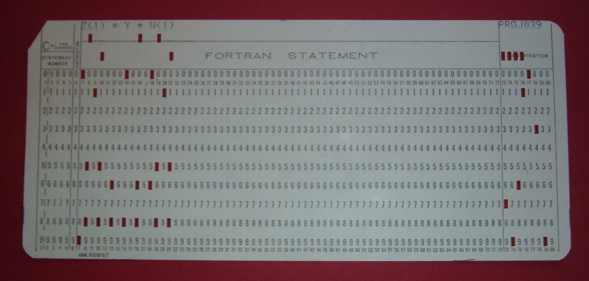
\includegraphics{images/chapter-1/perforated-card.png}
  \end{minipage}}
  \fbox{\begin{minipage}{\dimexpr \textwidth-2\fboxsep-2\fboxrule}
    \abovecaptionskip=0pt
    \caption{Perforated card}
  \end{minipage}}
\end{figure}

There are multiple lines on the card, each with varying holes. Each line describes a particular instruction that is necessary for the computations to be completed.

\begin{figure}[H]
  \lineskip=-\fboxrule
  \fbox{\begin{minipage}{\dimexpr \textwidth-2\fboxsep-2\fboxrule}
    \centering
    The user would describe their computations to someone who is capable of producing the correct perforated card needed for their computations.
    
	$\downarrow$
	
	The perforated card would be passed to the computer operator. A computer operator is a manager of computational resources that provides common services.
	
	$\downarrow$
	
	The computer operator would have a job queue from all of the users. These would be processed in a “first in, first out” (FIFO) fashion.
	
	$\downarrow$
	
	Jobs that are ready to be processed go in to batch processing. Each perforated card is passed through a computer system and the printed results are sent back to the user.
  \end{minipage}}
  \fbox{\begin{minipage}{\dimexpr \textwidth-2\fboxsep-2\fboxrule}
    \abovecaptionskip=0pt
    \caption{Process for performing computations in the 1950s}
  \end{minipage}}
\end{figure}


\section*{$>$1960s}

The process of performing computations after 1960 changed dramatically and required far less human input.

Automation was brought about by the “Operating System Paradigm” in which users could interface with a computer system directly through an operating system (OS).

\begin{figure}[H]
  \lineskip=-\fboxrule
  \fbox{\begin{minipage}{\dimexpr \textwidth-2\fboxsep-2\fboxrule}
    \centering
    \begin{tabular}{ccccc}
		User & $\rightarrow$ & Operating System (OS) & $\rightarrow$ & Results
	\end{tabular}
  \end{minipage}}
  \fbox{\begin{minipage}{\dimexpr \textwidth-2\fboxsep-2\fboxrule}
    \abovecaptionskip=0pt
    \caption{Process for performing computations after 1960}
  \end{minipage}}
\end{figure}


\section*{History details}

\begin{longtable}{|c|c|}
	\hline
	Late 1950s &
	\begin{minipage}[t]{0.8\textwidth}
    	\begin{itemize}
		    \item Standard subroutines were produced that were loaded at start-up. These contained features similar to those found on an operating system.
	  		\item Magnetic tapes were used for storage and were later replaced by disks.
	  		\item Assemblers started to be used. These are programs that takes basic computer instructions and convert them in to machine code; this is a pattern of binary bits (0’s and 1’s) that the computer system's processor can use to perform its basic operations.
	  		\item High-level languages, which consisted of more natural and human-readable language, started to be used. For example, FORTRAN is a general-purpose, compiled imperative programming language that is especially suited to numeric computation and scientific computing and was introduced in 1957.
    	\end{itemize}
  	\end{minipage}
	\\ \hline
	1960s &
	\begin{minipage}[t]{0.8\textwidth}
	  	Automated batch system.
	    \begin{itemize}
		    \item This replaced the computer operator.
		    \item Several programs could be loaded in to memory and automatically processed in a “first in, first out” (FIFO) fashion.
    	\end{itemize}
	\end{minipage}
	\\ \hline
	1970s &
	\begin{minipage}[t]{0.8\textwidth}
	  	Multiprogramming.
	    \begin{itemize}
		    \item The computer could switch between jobs, which allows processing and input/output (I/O) interaction simultaneously.
    	\end{itemize}
	\end{minipage}
	\\ \hline
	1980s &
	\begin{minipage}[t]{0.8\textwidth}
	  	Graphical user interfaces (GUIs).
	    \begin{itemize}
		    \item The interaction between a computer system and a user through the medium of a mouse and keyboard.
    	\end{itemize}
	\end{minipage}
	\\ \hline
\end{longtable}


\section{Hardware}

\section*{External hardware}

A \textbf{peripheral} is any external hardware device that provides input/output (I/O) for the computer.

For example, a keyboard and mouse are input peripherals, while a monitor and printer are output peripherals. Some peripherals, such as external hard drives, provide both input and output for the computer.

A computer system generally has many internal hardware components and hardware peripherals.

\begin{figure}[H]
  \lineskip=-\fboxrule
  \fbox{\begin{minipage}{\dimexpr \textwidth-2\fboxsep-2\fboxrule}
    \centering
    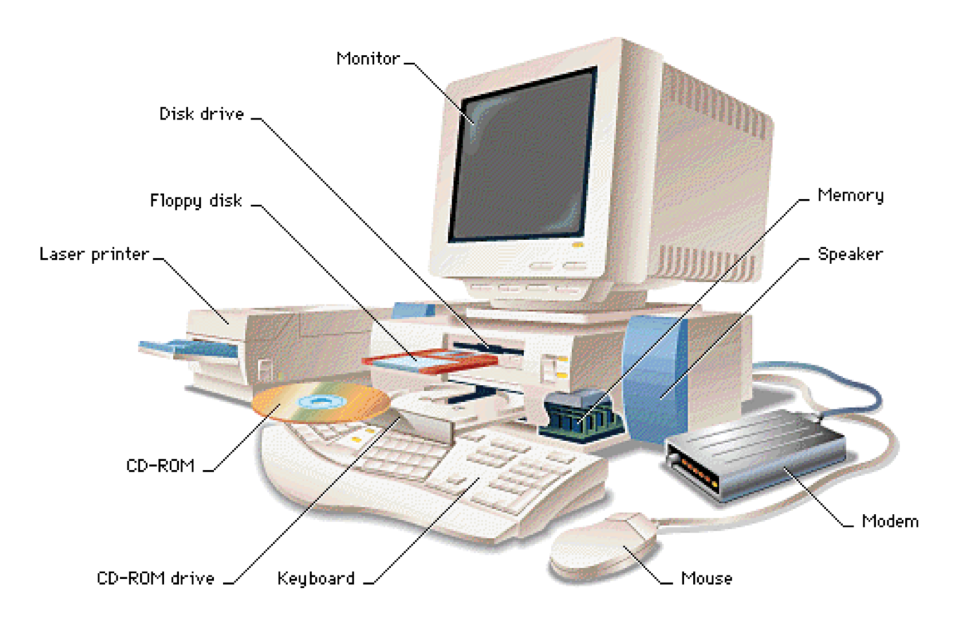
\includegraphics[max size={\textwidth}{\textheight}]{images/chapter-1/external-view-of-computer-system.png}
  \end{minipage}}
  \fbox{\begin{minipage}{\dimexpr \textwidth-2\fboxsep-2\fboxrule}
    \abovecaptionskip=0pt
    \caption{External view of computer system}
  \end{minipage}}
\end{figure}

\section*{Internal hardware}

A \textbf{processor} or \textbf{central processing unit (CPU)} is the hardware within a computer that carries out the instructions of a computer program by performing the basic arithmetical, logical, and input/output operations of the system.

A \textbf{motherboard} is the main printed circuit board (PCB) in a computer. The motherboard is a computer's central communications backbone connectivity point, through which all components and external peripherals connect.

Inside of a computer system, there are many components connected to the processor via the motherboard.

\begin{figure}[H]
  \lineskip=-\fboxrule
  \fbox{\begin{minipage}{\dimexpr \textwidth-2\fboxsep-2\fboxrule}
    \centering
    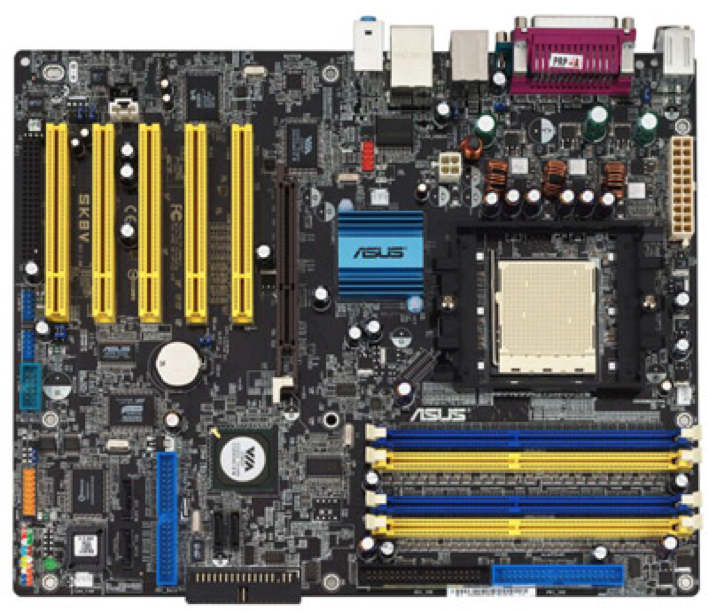
\includegraphics[max size={\textwidth}{\textheight}]{images/chapter-1/typical-computer-motherboard.png}
  \end{minipage}}
  \fbox{\begin{minipage}{\dimexpr \textwidth-2\fboxsep-2\fboxrule}
    \abovecaptionskip=0pt
    \caption{Typical computer motherboard}
  \end{minipage}}
\end{figure}

The motherboard connects:
\begin{itemize}
	\item all of the internal components via the data bus; and
	\item the peripherals.
\end{itemize}


\section{What is an operating system (OS)?}

\section*{Definition}

An \textbf{operating system (OS)} is a collection of system programs that manage the hardware resources and peripherals connected to a computer system. It is also responsible for the graphical user interface or command line interface and all other software running on the computer system.


\section*{Purpose of an operating system (OS)}

An operating system (OS) is designed to:
\begin{itemize}
	\item eliminate the need to have hardware knowledge to operate a computer system;
	\item make the boundary between hardware and software transparent, allowing the user to not be concerned with the technical details; and
	\item provide a user-friendly environment to execute and develop programs.
\end{itemize}

These attributes are achieved by layering the computer system such that the user can interface with applications, rather than the operating system (OS) or the hardware directly.

\begin{figure}[H]
  \lineskip=-\fboxrule
  \fbox{\begin{minipage}{\dimexpr \textwidth-2\fboxsep-2\fboxrule}
    \centering
    User
    
	$\updownarrow$
	
	Applications
	
	$\updownarrow$
	
	Operating System (OS)
	
	$\updownarrow$
	
	Computer System Hardware
  \end{minipage}}
  \fbox{\begin{minipage}{\dimexpr \textwidth-2\fboxsep-2\fboxrule}
    \abovecaptionskip=0pt
    \caption{Computer system layers}
  \end{minipage}}
\end{figure}


\section*{Structure of an operating system (OS)}

The structure of an operating system (OS) can be said to resemble an onion.

\begin{figure}[H]
  \lineskip=-\fboxrule
  \fbox{\begin{minipage}{\dimexpr \textwidth-2\fboxsep-2\fboxrule}
    \centering
    
\includegraphics[max size={\textwidth}{\textheight}]{images/chapter-1/structure-of-an-os.png}
  \end{minipage}}
  \fbox{\begin{minipage}{\dimexpr \textwidth-2\fboxsep-2\fboxrule}
    \abovecaptionskip=0pt
    \caption{Structure of an operating system (OS)}
  \end{minipage}}
\end{figure}

An operating system (OS) has four main components.

The \textbf{kernel} hides the complexity of how a computer system works from users. It is responsible for:
\begin{itemize}
	\item process management;
	\item CPU scheduling; and
	\item handling interrupts.
\end{itemize}

\textbf{Memory management} is responsible for allocating and deallocating memory to processes.

\textbf{Input/output (I/O)} includes any interaction between the internal computer system components and peripherals.

The \textbf{filing system} is comprised of file management subsystems.

Each layer in the operating system (OS) structure provides functions to the above layers. Each layer uses facilities provided by layers within and below that layer. 


\section*{Practical features of current operating systems (OSs)}

\begin{longtable}{|c|c|}
	\hline
	Concurrency &
	\begin{minipage}[t]{0.6\textwidth}
	Allows overlapping input/output (I/O) operations with computations and several programs to be stored in memory at a single time.
	\end{minipage}
	\\ \hline
	Sharing of resources &
	\begin{minipage}[t]{0.6\textwidth}
	Sharing hardware and peripherals, such as hard disks and printers.
	\end{minipage}
	\\ \hline
	Access to long term storage &
	\begin{minipage}[t]{0.6\textwidth}
	Important for saving important files on mediums such as hard disk drives (HDDs) and solid-state drives (SSDs).
	\end{minipage}
	\\ \hline
	Non-determinacy &
	\begin{minipage}[t]{0.6\textwidth}
	The ability to cope with unpredictable events without crashing.
	\end{minipage}
	\\ \hline
\end{longtable}


\section{Functions of an operating system}

An operating system (OS) has two main complementary functions:
\begin{itemize}
	\item resource managing; and
	\item machine extending.
\end{itemize}


\section*{Resource managing}

It manages resources shared among users and user programs and maximises their utilisation of the CPU, RAM and other resources. This is done simultaneously in order to increase the availability.

This is similar to the role of computer operators in the 1950s.


\section*{Machine extending}

It presents a virtual machine (or extended machine) to users that is much easier to access than the underlying physical machine.

\begin{figure}[H]
  \lineskip=-\fboxrule
  \fbox{\begin{minipage}{\dimexpr \textwidth-2\fboxsep-2\fboxrule}
    \centering
    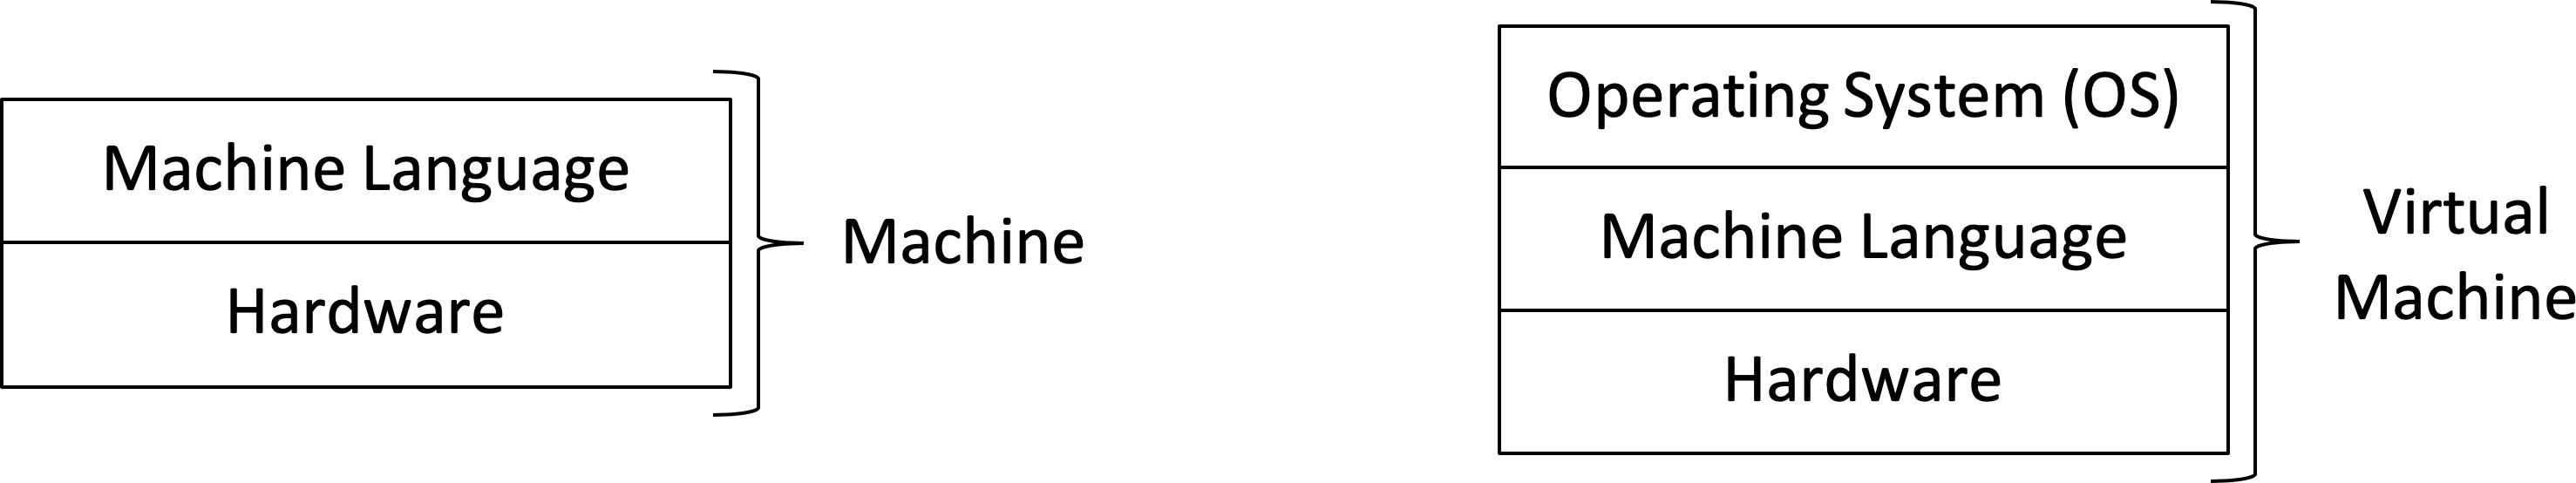
\includegraphics[max size={\textwidth}{\textheight}]{images/chapter-1/machine-extending.png}
  \end{minipage}}
  \fbox{\begin{minipage}{\dimexpr \textwidth-2\fboxsep-2\fboxrule}
    \abovecaptionskip=0pt
    \caption{Machine extending}
  \end{minipage}}
\end{figure}

The virtual machine presented to the user provides an abstraction of the computer system. This hides the complexity of the hardware from the user; this means that the user need only be concerned with the details of the hardware if they desire.

This is a way of translating the functions needed by a user from the hardware to a presentable and user-friendly medium. As a result, the operating system (OS) acts as an intermediary layer between the user and machine language.

The benefit of this abstraction can be demonstrated when comparing how computations may be processed with and without an operating system (OS).

\begin{figure}[H]
  \lineskip=-\fboxrule
  \fbox{\begin{minipage}{\dimexpr \textwidth-2\fboxsep-2\fboxrule}
    \begin{longtable}{|c|c|}
    	\hline
		\textbf{Without Operating System (OS)} & \textbf{With Operating System (OS)} \\
		\hline
		\begin{minipage}[t]{0.45\textwidth}
	    	The instructions written in machine code or assembly language much interface directly with memory hardware. As such, the memory locations to load the two numbers from must be explicitly defined and the memory location to which the result is stored must also be defined.
	    	
			The example below shows a possible assembly code implementation of a computation that is capable of adding two numbers.
	  	\end{minipage}
		&
		\begin{minipage}[t]{0.45\textwidth}
	    	The instructions can be written in a high-level language, such as C++.
	  	\end{minipage}
		\\ \hline
		\begin{minipage}[t]{0.45\textwidth}
			\begin{tabular}{p{2cm} | p{3.5cm}}
				\hline
				LDAA \$80 & (load number at memory location 80) \\
				\hline
				LDAB \$81 & (load number at memory location 81) \\
				\hline
				ADDB & (add these two numbers) \\
				\hline
				STAA \&55 & (store the sum to memory location 55) \\
				\hline
			\end{tabular}
	  	\end{minipage}
		&
		\begin{minipage}[t]{0.45\textwidth}
	    	int a, b, c;
	    	
			a = 1;
			
			b = 2;
			
			c = a + b;
	  	\end{minipage}
	\end{longtable}
	
  \end{minipage}}
  \fbox{\begin{minipage}{\dimexpr \textwidth-2\fboxsep-2\fboxrule}
    \abovecaptionskip=0pt
    \caption{Adding two numbers}
  \end{minipage}}
\end{figure}

This demonstrates that program development is much more user-friendly with an operating system (OS). This is because without an operating system (OS) the user must have knowledge of the system hardware; in this case, the necessary memory locations.

In addition, it is possible that the machine code or assembly language written may not work on another computer system as that computer system may have a different architecture or the memory locations may be different. For example, in another computer system:
\begin{itemize}
	\item memory location 81 may not exist as the memory is smaller; or
	\item memory location 55 contains important data or instructions that should not be overwritten and therefore the computer system may crash.
\end{itemize}

By contrast, with an operating system (OS), it is possible to perform computations without interfacing directly with hardware. In the example above, variables (a, b and c) can be used to access data in memory rather than addressing memory locations. The only concern here is that the variable c is able to store the result of a + b.

The operating system (OS) provides a unified environment to users to run their computations in different systems. The operating system (OS) is capable of taking high-level code and translating it in to the machine code that can be executed on a particular computer system.


\section{Current operating system (OS) trends}

\section*{Hardware evolution}

Due to fast rate of hardware evolution, operating systems (OSs) are more wide-spread than just traditional desktop computers. They can be found on hardware such as:
\begin{itemize}
	\item mobile devices, such as smartphones and tablets; and
	\item embedded systems.
\end{itemize}

\begin{figure}[H]
  \lineskip=-\fboxrule
  \fbox{\begin{minipage}{\dimexpr \textwidth-2\fboxsep-2\fboxrule}
    \begin{longtable}{|c|c|c|}
    	\hline
		\textbf{Desktop} & \textbf{Mobile} & \textbf{Embedded} \\
		\hline
		\begin{minipage}[t]{0.26\textwidth}
	    	\begin{itemize}
	    		\item Windows
	    		\item macOS
	    		\item Linux
	    	\end{itemize}
	  	\end{minipage}
		&
		\begin{minipage}[t]{0.26\textwidth}
	    	\begin{itemize}
	    		\item iOS
	    		\item Android
	    		\item Symbian OS
	    	\end{itemize}
	  	\end{minipage}
		&
		\begin{minipage}[t]{0.26\textwidth}
	    	\begin{itemize}
	    		\item Windows Embedded
	    	\end{itemize}
	  	\end{minipage}
	  	\\ \hline
	\end{longtable}
  \end{minipage}}
  \fbox{\begin{minipage}{\dimexpr \textwidth-2\fboxsep-2\fboxrule}
    \abovecaptionskip=0pt
    \caption{Popular operating systems (OSs)}
  \end{minipage}}
\end{figure}


\section*{Multiprocessor systems}

\subsection*{Definiton}

A \textbf{multiple processor computer system} makes use of two or more processors and has the ability to allocate tasks between them.


\subsection*{Workstations}

A single machine may contain multiple processors and therefore have large computing power.


\subsection*{Distributed and network systems}

These computer systems share computing power and peripherals.

\begin{figure}[H]
  \lineskip=-\fboxrule
  \fbox{\begin{minipage}{\dimexpr \textwidth-2\fboxsep-2\fboxrule}
    \centering
    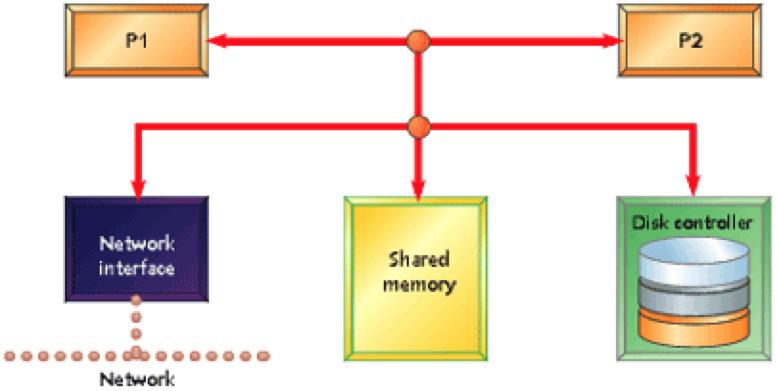
\includegraphics[max size={\textwidth}{\textheight}]{images/chapter-1/distributed-and-network-systems.png}
  \end{minipage}}
  \fbox{\begin{minipage}{\dimexpr \textwidth-2\fboxsep-2\fboxrule}
    \abovecaptionskip=0pt
    \caption{Distributed and network systems}
  \end{minipage}}
\end{figure}

The diagram shows an abstraction of a distributed or network system. P1 and P2 are the connected computer systems that both share memory, access to the disk control and, if the system is a network system, the network interface.

However, there is a distinguishable difference between distributed and network systems.

\begin{longtable}{|c|c|}
	\hline
	\textbf{Similarities} & \textbf{Differences} \\
	\hline
	\begin{minipage}[t]{0.45\textwidth}
		Consist of multiple systems that are interconnected to exchange information.
	\end{minipage}
	&
	\begin{minipage}[t]{0.45\textwidth}
		In distributed systems, users are not aware of the multiplicity of computer systems available.
	\end{minipage}
	\\ \hline
	&
	\begin{minipage}[t]{0.45\textwidth}
		In network systems, users explicitly move/share files, submit jobs for processing and other perform other similar tasks.
	\end{minipage}
	\\ \hline
	&
	\begin{minipage}[t]{0.45\textwidth}
		In distributed systems, tasks such as moving/sharing files, submitting jobs for processing and other similar tasks are handled automatically by the operating system (OS).
	\end{minipage}
	\\ \hline
\end{longtable}


\subsection*{Evaluation}

\begin{longtable}{|c|c|}
	\hline
	\textbf{Advantages} & \textbf{Disadvantages} \\
	\hline
	\begin{minipage}[t]{0.45\textwidth}
		\textbf{Increase processor throughput} due to the use of parallel processing.
	\end{minipage}
	&
	\begin{minipage}[t]{0.45\textwidth}
		\textbf{A more complex operating system is required} in order to be able to interface and manage multiple processor units.
	\end{minipage}
	\\ \hline
	\begin{minipage}[t]{0.45\textwidth}
		\textbf{Lower cost} than using multiple processors across multiple computer systems because the processors share resources such as the power supply and motherboard.
	\end{minipage}
	&
	\\ \hline
	\begin{minipage}[t]{0.45\textwidth}
		\textbf{Increased reliability} because failure of one processor does not affect the other processors and will only slow down the computer system.
	\end{minipage}
	&
	\\ \hline
\end{longtable}


\section{Operating system (OS) layers}

\section*{User interfaces}

In an operating system (OS), the top layer is the user interface. This is the only layer explicitly visible to the user.

The user interface may be a:
\begin{longtabu} to \textwidth {X[6,l] X[1,c] X[10,l]}
	\textbullet terminal & -- & text-based command prompt; and/or
	\\
	\textbullet graphical user interface (GUI) & -- & a visual way of interacting with a computer using items such as windows, icons and menus.
\end{longtabu}


\subsection*{History of the graphical user interface (GUI)}

The first company to develop a graphical user interface (GUI) was Xerox PARC. They developed the “Alto” personal computer. It had a bitmapped screen and was the first computer to have a “desktop” screen with a graphical user interface (GUI).

The “Alto” personal computer was not a commercial product. However, several thousand units were manufactured and used at Xerox’s offices and several universities.

This development was a large influence on the design of personal computers during the late 1970s and early 1980s. Notable examples include:
\begin{itemize}
	\item Three Rivers PERQ;
	\item Apple Lisa;
	\item Apple Macintosh; and
	\item the first Sun Workstations.
\end{itemize}


\section{Kernel mode}

\section*{Kernel mode vs user mode}

\begin{longtabu} to \textwidth {| X[1,l] | X[1,l] |}
    \hline
    \textbf{Kernel Mode} & \textbf{User Mode}
    \\ \hline
    Operating systems (OSs) run in kernel mode.
    
    This allows:
    \begin{itemize}
    	\item execution of privileged machine instructions; and
    	\item complete access and control of all the hardware.
    \end{itemize}
    &
    Other software runs in user mode.

	In this mode, instructions that affect control of the machine are forbidden.

	For example:
	\begin{itemize}
		\item 	web browsers;
		\item e-mail software; and
		\item music players.
	\end{itemize}
	\\ \hline
\end{longtabu}

\begin{figure}[H]
  \lineskip=-\fboxrule
  \fbox{\begin{minipage}{\dimexpr \textwidth-2\fboxsep-2\fboxrule}
    \centering
    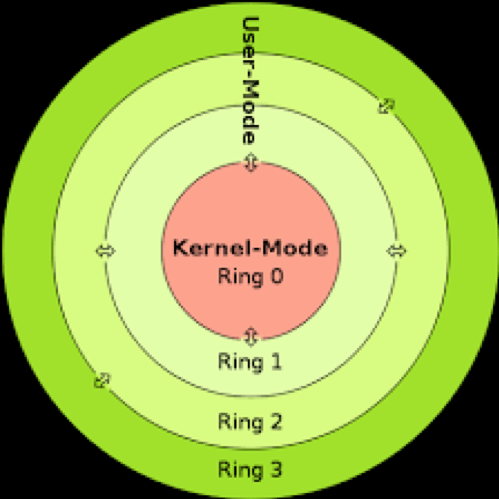
\includegraphics[max size={\textwidth}{\textheight}]{images/chapter-1/kernel-mode-and-user-mode.png}
  \end{minipage}}
  \fbox{\begin{minipage}{\dimexpr \textwidth-2\fboxsep-2\fboxrule}
    \abovecaptionskip=0pt
    \caption{Kernel mode and user mode}
  \end{minipage}}
\end{figure}

Ring 0 represents the kernel mode.

Rings 1-3 represent the user mode.


\section*{Kernel mode protection}

These rings allow separation between the operating system (OS) and user programs for security and protection purposes.

If user mode had unrestricted access to all of the machine instructions:
\begin{itemize}
	\item a user could inadvertently obtain a virus or write code that is capable of causing damage to the system, and therefore it is necessary to prevent any instructions from directly controlling the machine;
	\item a program may use resources unfairly, such as holding the CPU or memory, and therefore harm the execution of other programs; and/or
	\item sensitive machine instructions could be used improperly which may lead to kernel mode errors.
\end{itemize}

Kernel mode errors are catastrophic.


\begin{figure}[H]
  \lineskip=-\fboxrule
  \fbox{\begin{minipage}{\dimexpr \textwidth-2\fboxsep-2\fboxrule}
    \begin{longtabu} to \textwidth {| X[1,l] | X[1,l] |}
	    \hline
	    \textbf{Kernel Mode} & \textbf{User Mode}
	    \\ \hline
	    A kernel panic represents the operating system (OS) attempting to prevent software causing any harm to the computer system and to recover from a kernel mode error on reboot.
	    
	    An example of a kernel panic is the “Blue Screen of Death” (BSoD) in Microsoft’s Windows.
	    &
	    Application errors where an exception was thrown due to an attempt to execute a privileged instruction, this is one that should only be accessed and executed by the kernel mode, represents the operating system (OS) preventing an application from having unrestricted access to all of the machine instructions.
		\\ \hline
		\centering
    	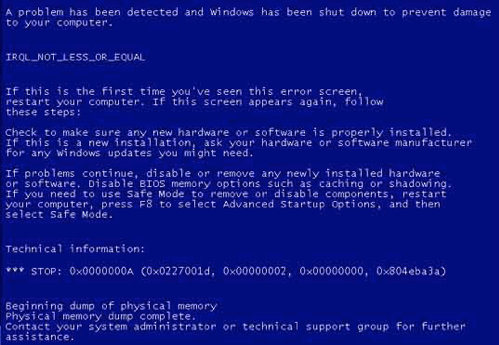
\includegraphics[max size={0.45\textwidth}{\textheight}]{images/chapter-1/kernel-mode-error-bsod.png}
	    &
	    \centering
    	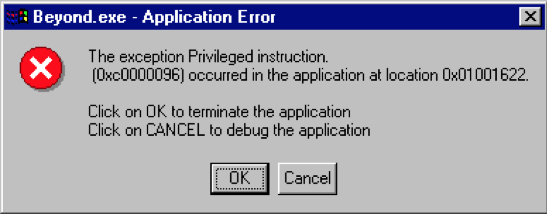
\includegraphics[max size={0.45\textwidth}{\textheight}]{images/chapter-1/kernel-mode-error-application-error.png}
		\\ \hline
	\end{longtabu}
  \end{minipage}}
  \fbox{\begin{minipage}{\dimexpr \textwidth-2\fboxsep-2\fboxrule}
    \abovecaptionskip=0pt
    \caption{Kernel mode errors}
  \end{minipage}}
\end{figure}


\section*{System calls}

A \textbf{system call} is the programmatic way in which a computer program requests a service from the kernel of the operating system on which it is executed. A system call is a way for programs to interact with the operating system.

Some privileged instructions can be called by a programmer via system calls. Operating systems (OSs) contain system calls for which provide a layer of services for user programs to implement some activities/request services. These are usually sensitive or privileged from the kernel.

All interactions with the hardware are implemented via system calls. For example, a system call may occur if an application requires interaction with a peripheral such as a printer.

Invoking a system call is similar to calling a general function. However, the difference is that a general function’s code is part of program itself, while the system call code is part of the operating system (OS). Different operating systems (OSs) offer different (limited) sets of system calls.

\begin{figure}[H]
  \lineskip=-\fboxrule
  \fbox{\begin{minipage}{\dimexpr \textwidth-2\fboxsep-2\fboxrule}
    \begin{longtabu} to \textwidth {| X[1,l] | X[2,l] |}
	    \hline
	    \textbf{Call} & \textbf{Description}
	    \\ \hline
	    \multicolumn{2}{|c|}{\textbf{Process Mangament}}
	    \\ \hline
	    pid = fork()
	    &
	    Create a child process identical to the parent.
		\\ \hline
		exit(status)
	    &
	    Terminate process execution and return status.
		\\ \hline
		\multicolumn{2}{|c|}{\textbf{File Mangament}}
	    \\ \hline
	    n = read(fd, buffer, nbytes)
	    &
	    Read data from a file in to a buffer.
		\\ \hline
		n = write(fd, buffer, nbytes)
	    &
	    Write data to a file
		\\ \hline
		\multicolumn{2}{|c|}{\textbf{Process Mangament}}
	    \\ \hline
	    seconds = time(\&seconds)
	    &
	    Get the elapsed time since Jan 1. 1970
		\\ \hline
	\end{longtabu}
  \end{minipage}}
  \fbox{\begin{minipage}{\dimexpr \textwidth-2\fboxsep-2\fboxrule}
    \abovecaptionskip=0pt
    \caption{Unix system calls}
  \end{minipage}}
\end{figure}


\chapter{Process Management}

\section{Programs and processes}

\section*{Definitions}

A \textbf{program} is the code written by a programmer.

A \textbf{process} (or job/task) shows a program in execution and is a particular instance of a program. These many be shown in a monitoring software, such as Windows Task Manager.

\textbf{Data} are stored values used for the computations by the process.


\section*{How it works}

A single program may have multiple processes that are currently running.

Each process can share the same code for the program. This is possible as each process uses its own address space, a list of memory locations which the process can read and write. These memory locations contain the program’s code instructions and data.

A program is only code however, once it is run, a process is started, and it becomes instructions and data.

\begin{figure}[H]
  \lineskip=-\fboxrule
  \fbox{\begin{minipage}{\dimexpr \textwidth-2\fboxsep-2\fboxrule}
    \centering
    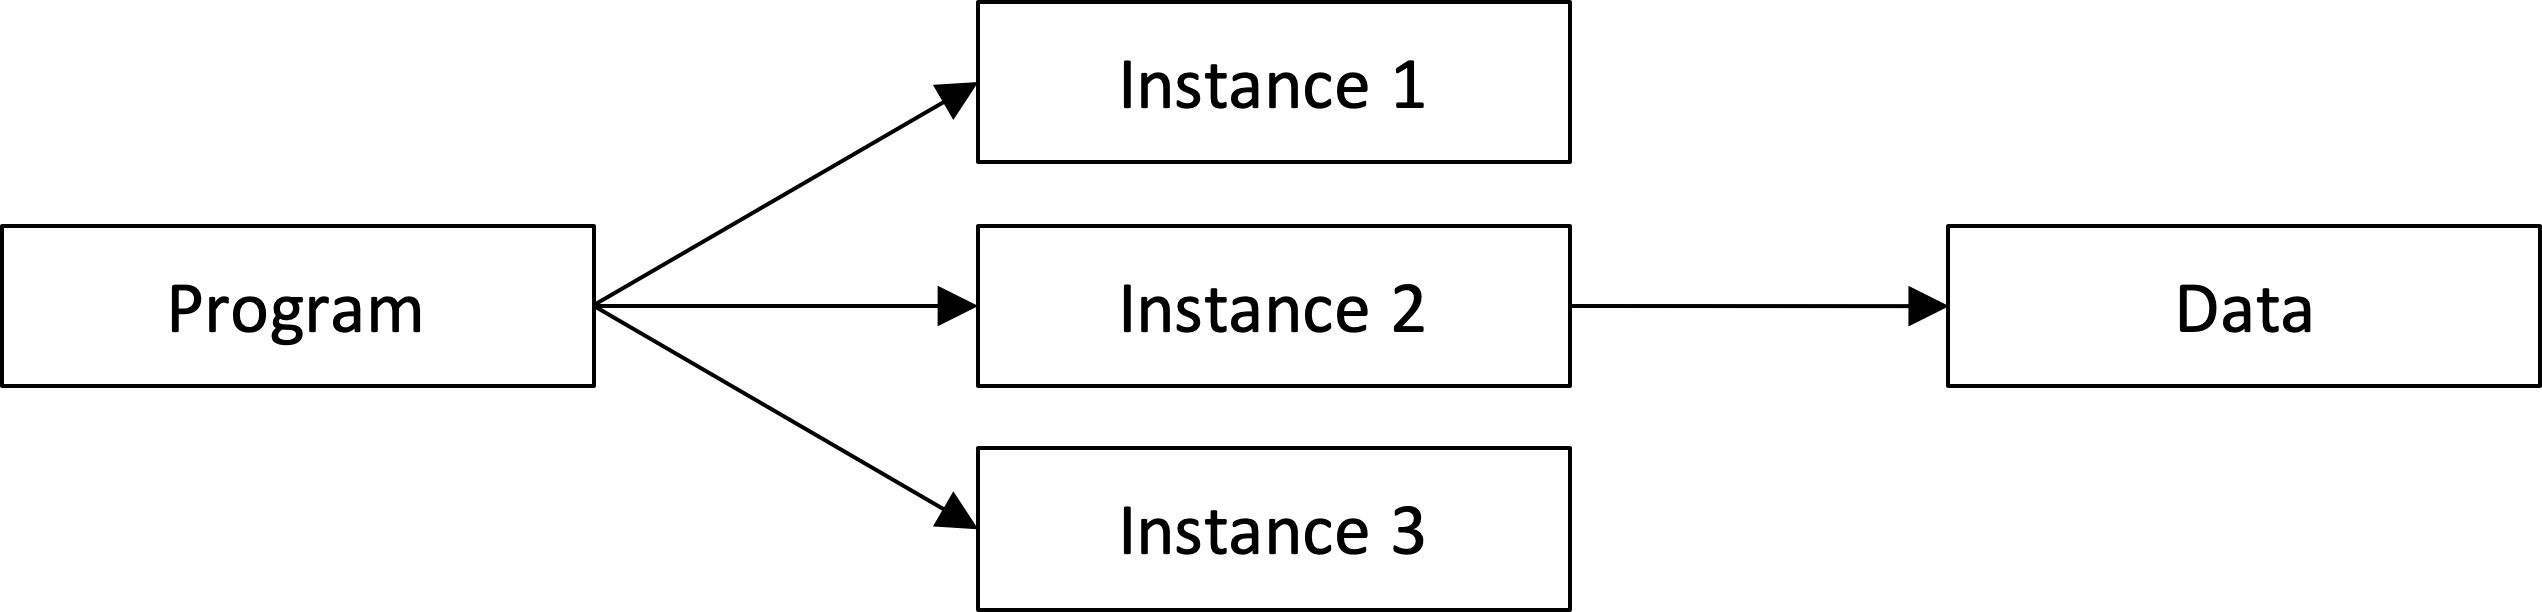
\includegraphics[max size={\textwidth}{\textheight}]{images/chapter-2/programs-and-processes.png}
  \end{minipage}}
  \fbox{\begin{minipage}{\dimexpr \textwidth-2\fboxsep-2\fboxrule}
    \abovecaptionskip=0pt
    \caption{Programs and processes}
  \end{minipage}}
\end{figure}


\section{Process life cycle}

\section*{Process creation}

A process can be created by:

\begin{longtabu} to \textwidth {X[3,l] X[1,c] X[10,l]}
	\textbullet a user & -- & a program may be executed by a user, such as via a double-click using a graphical user interface (GUI) or by typing in a command, and “trigger” the processor to load the program’s executable file containing the program code; or
	\\
	\textbullet another process & -- & an existing process may create another process by spawning/forking – the process that creates a new process is called the parent process while the new process is called the child process. The child process may also spawn a new process forming a tree of processes, as demonstrated in the diagram below.
\end{longtabu}

\begin{figure}[H]
  \lineskip=-\fboxrule
  \fbox{\begin{minipage}{\dimexpr \textwidth-2\fboxsep-2\fboxrule}
    \centering
    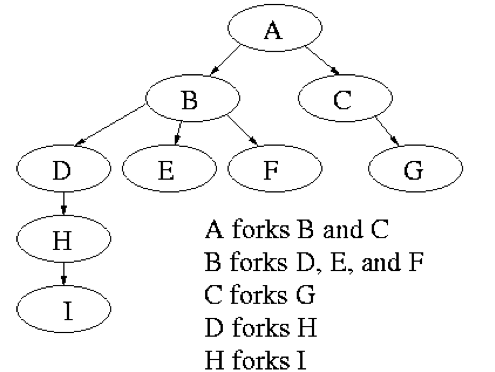
\includegraphics[max size={\textwidth}{\textheight}]{images/chapter-2/process-creation.png}
  \end{minipage}}
  \fbox{\begin{minipage}{\dimexpr \textwidth-2\fboxsep-2\fboxrule}
    \abovecaptionskip=0pt
    \caption{Process creation}
  \end{minipage}}
\end{figure}


\section*{Process table and process control block}

A \textbf{process identification number (PID)} is a unique identifier given to a new process when it is created.

A \textbf{process control block (PCB)} holds all of the information about a process. It is created when new process is created.

A \textbf{process table} stores the process identification numbers (PIDs) for a process and a pointer to the respective process control block (PCB) for that process. This is managed by the operating system (OS).

\begin{figure}[H]
  \lineskip=-\fboxrule
  \fbox{\begin{minipage}{\dimexpr \textwidth-2\fboxsep-2\fboxrule}
    \centering
    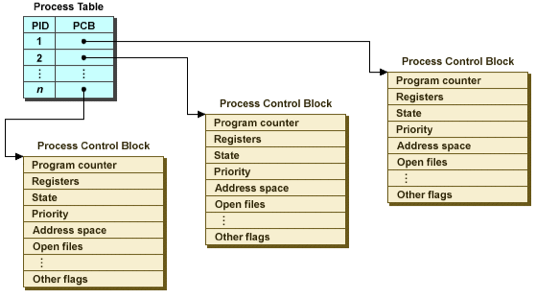
\includegraphics[max size={\textwidth}{\textheight}]{images/chapter-2/process-table.png}
  \end{minipage}}
  \fbox{\begin{minipage}{\dimexpr \textwidth-2\fboxsep-2\fboxrule}
    \abovecaptionskip=0pt
    \caption{Process table with respective process control blocks}
  \end{minipage}}
\end{figure}

The process descriptor fields in the process control block (PCB) may differ between operating system (OS). An example of possible process descriptor fields is shown by those used by the Minix operating system (OS) are shown below.

\begin{figure}[H]
  \lineskip=-\fboxrule
  \fbox{\begin{minipage}{\dimexpr \textwidth-2\fboxsep-2\fboxrule}
    \begin{longtabu} to \textwidth {X[2,l] X[2,l] X[2,l]}
	    \hline
	    \textbf{Process Management} & \textbf{Memory Management} & \textbf{File Management}
	    \\ \hline
	    Registers & Pointer to text segment	& UMASK mask
		\\ \hline
		Program counter & Pointer to data segment & Root directory
		\\ \hline
		Program status word & Pointer to bss segment & Working directory
		\\ \hline
		Stack pointer & Exit status & File descriptors
		\\ \hline
		Process state & Signal status & Effective uid
		\\ \hline
		Time when process started & Process ID & Effective gid
		\\ \hline
		CPU time used & Parent process & System call parameters
		\\ \hline
		Children’s CPU time & Process group & Various flag bits
		\\ \hline
		Time of next alarm & Real uid &
		\\ \hline
		Message queue pointers & Effective uid &
		\\ \hline
		Pending signal bits & Real gid &
		\\ \hline
		Process ID & Effective gid &
		\\ \hline
		Various flag bits & Various flag bits &
		\\ \hline
	\end{longtabu}
  \end{minipage}}
  \fbox{\begin{minipage}{\dimexpr \textwidth-2\fboxsep-2\fboxrule}
    \abovecaptionskip=0pt
    \caption{Process descriptor fields in Minix}
  \end{minipage}}
\end{figure}

Although Minix is a fully-featured operating system (OS), it is a small operating system (OS) and therefore the processor descriptor fields are less complex than other operating systems (OSs).


\section*{Three-state model}

The \textbf{three-state model} shows how a process, once initiated, can be in one of three states. The current state of a process is stored in its respective process control block (PCB).

A process, once initiated, can be in one of three main states:
\begin{longtabu} to \textwidth {X[2,l] X[1,c] X[10,l]}
	\textbullet running & -- & actually using the CPU to perform a task;
	\\
	\textbullet ready & -- & ready to run but waiting for the CPU as it has not yet had time on the CPU has been temporarily stopped to let another process run; or
	\\
	\textbullet ready & -- & unable to run until some external event occurs, such as:
		\begin{itemize}
			\item waiting for an interrupt, this is a message from the hardware saying that a resource is now available to read from – such as waiting for an input/output (I/O) operation to complete; and
			\item waiting for another process to finish accessing a shared resources – for example: a file; memory; or an external peripheral, such as a printer.
		\end{itemize}
\end{longtabu}

\begin{figure}[H]
  \lineskip=-\fboxrule
  \fbox{\begin{minipage}{\dimexpr \textwidth-2\fboxsep-2\fboxrule}
    \centering
    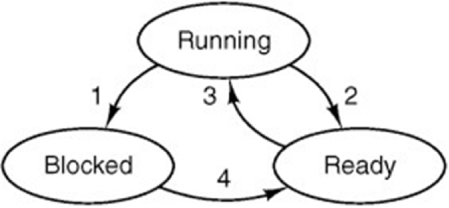
\includegraphics[max size={\textwidth}{\textheight}]{images/chapter-2/process-states.png}
  \end{minipage}}
  \fbox{\begin{minipage}{\dimexpr \textwidth-2\fboxsep-2\fboxrule}
    \abovecaptionskip=0pt
    \caption{Process states}
  \end{minipage}}
\end{figure}

In reference to the diagram above, transitions can occur between process states.

\begin{figure}[H]
  \lineskip=-\fboxrule
  \fbox{\begin{minipage}{\dimexpr \textwidth-2\fboxsep-2\fboxrule}
    \begin{longtabu} to \textwidth {|X[4,l]|X[1.5,l]|X[6,l]|}
	    \hline
	    \textbf{Transition} & \textbf{Diagram Number} & \textbf{Explanation}
	    \\ \hline
	    \textbf{running $\rightarrow$ blocked}
	    & \textbf{1} &
	    \textbf{Process blocks for input.}
	    
		For example, if the process is waiting for some input from I/O.
		\\ \hline
		\textbf{running $\rightarrow$ ready}
	    & \textbf{2} &
	    \textbf{Scheduler picks another process.}
	    
		The process has had opportunity to run and is flagged as no longer currently running, so that another process can run.
		\\ \hline
		\textbf{ready $\rightarrow$ running}
	    & \textbf{3} &
	    \textbf{Scheduler picks this process.}
		The next process that is ready to run is set to running to allow access to the CPU.
		\\ \hline
		\textbf{blocked $\rightarrow$ ready}
	    & \textbf{4} &
	    \textbf{Input becomes available.}
		The process has received input from I/O or the process sends an interrupt and the interrupt service routine (ISR) is executed, the scheduler is called to transition the process from blocked to ready.
		\\ \hline
	\end{longtabu}
  \end{minipage}}
  \fbox{\begin{minipage}{\dimexpr \textwidth-2\fboxsep-2\fboxrule}
    \abovecaptionskip=0pt
    \caption{Transitions between processor states}
  \end{minipage}}
\end{figure}

The transition between process states is dependent on the scheduling algorithm used. A clock is used to send a signal to stop the current process, move it from running to ready and then run the scheduler to find out what process should be processed next and the next process will be made to running.


\section*{State queues}

At any time, a process is in only one state.


\subsection*{Running processes}

At any time, at most one process is in the running state. This is because a single-core processor is only able to process one instruction coming from a single core at a time. If a computer system has a multi-core processor, this rule applies to each individual core on the processor, rather than the processor as a whole, as they are able to complete parallel execution.

\begin{figure}[H]
  \lineskip=-\fboxrule
  \fbox{\begin{minipage}{\dimexpr \textwidth-2\fboxsep-2\fboxrule}
    \centering
    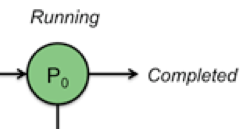
\includegraphics[max size={\textwidth}{\textheight}]{images/chapter-2/running-processes.png}
  \end{minipage}}
  \fbox{\begin{minipage}{\dimexpr \textwidth-2\fboxsep-2\fboxrule}
    \abovecaptionskip=0pt
    \caption{Running processes}
  \end{minipage}}
\end{figure}


\subsection*{Ready processes}

There may be a queue of processes in the ready state.

\begin{figure}[H]
  \lineskip=-\fboxrule
  \fbox{\begin{minipage}{\dimexpr \textwidth-2\fboxsep-2\fboxrule}
    \centering
    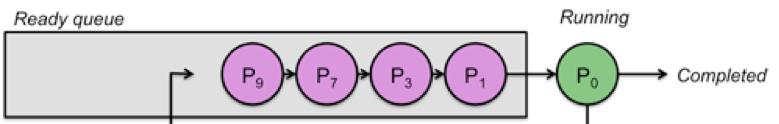
\includegraphics[max size={\textwidth}{\textheight}]{images/chapter-2/ready-processes.png}
  \end{minipage}}
  \fbox{\begin{minipage}{\dimexpr \textwidth-2\fboxsep-2\fboxrule}
    \abovecaptionskip=0pt
    \caption{Ready processes}
  \end{minipage}}
\end{figure}


\subsection*{Blocked processes}

There may be several queues of processes in the blocked state, where each queue represents one resource for which processes in that queue are waiting.

\begin{figure}[H]
  \lineskip=-\fboxrule
  \fbox{\begin{minipage}{\dimexpr \textwidth-2\fboxsep-2\fboxrule}
    \centering
    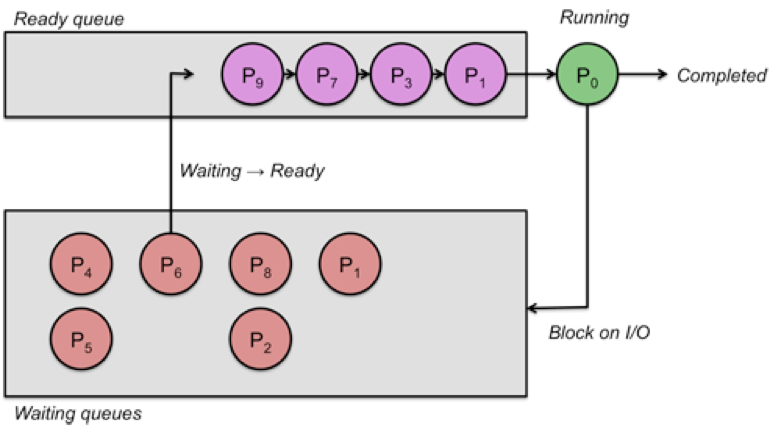
\includegraphics[max size={\textwidth}{\textheight}]{images/chapter-2/currently-running-processes.png}
  \end{minipage}}
  \fbox{\begin{minipage}{\dimexpr \textwidth-2\fboxsep-2\fboxrule}
    \abovecaptionskip=0pt
    \caption{Currently running processes}
  \end{minipage}}
\end{figure}


\section*{Process termination}

\textbf{Process termination} is the end of life for a process, this can occur in two general ways.


\subsection*{Voluntary termination}

\textbf{Voluntary termination} of a process represents the end of life for a process where its termination was intended by the user or the programmer.

This can be a:
\begin{longtabu} to \textwidth { X[1.5,l] X[0.2,l] X[7,l]}
	\textbf{\textbullet normal exit}
	& -- &
	the process has done its work; or
	\\
	\textbf{\textbullet error exit}
	& -- &
	the process itself handles and “catches” an error – for example, some try-catch code is implemented to check if a condition is met, such as if the definition of a variable is present.
\end{longtabu}

\begin{figure}[H]
  \lineskip=-\fboxrule
  \fbox{\begin{minipage}{\dimexpr \textwidth-2\fboxsep-2\fboxrule}
    \centering
    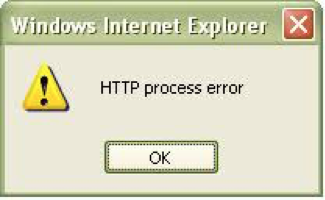
\includegraphics[max size={\textwidth}{\textheight}]{images/chapter-2/voluntary-termination.png}
  \end{minipage}}
  \fbox{\begin{minipage}{\dimexpr \textwidth-2\fboxsep-2\fboxrule}
    \abovecaptionskip=0pt
    \caption{Voluntary termination due to an error exit}
  \end{minipage}}
\end{figure}


\subsection*{Involuntary termination}

\textbf{Involuntary termination} of a process represents the end of life for a process where its termination as not intended by the user or the programmer.

This can be due to:
\begin{longtabu} to \textwidth { X[1.5,l] X[0.2,l] X[7,l]}
	\textbf{\textbullet a fatal error}
	& -- &
	an error is detected by the operating system’s (OS’s) protected mode – for example, an exception has been thrown due to reference to a non-existent memory location or division by zero; or
	\\
	\textbf{\textbullet being killed by another process}
	& -- &
	a process may execute a system call that causes the operating system (OS) to kill another process – this process may have control over the killed process and this may be due to that process being the parent process of the killed process.
\end{longtabu}

\begin{figure}[H]
  \lineskip=-\fboxrule
  \fbox{\begin{minipage}{\dimexpr \textwidth-2\fboxsep-2\fboxrule}
    \centering
    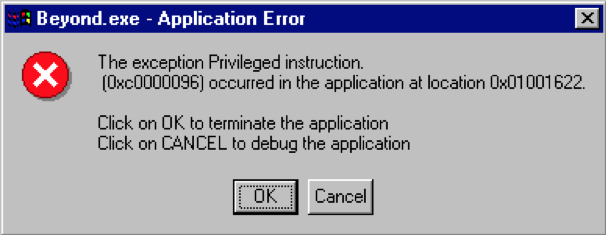
\includegraphics[max size={\textwidth}{\textheight}]{images/chapter-2/involuntary-termination.png}
  \end{minipage}}
  \fbox{\begin{minipage}{\dimexpr \textwidth-2\fboxsep-2\fboxrule}
    \abovecaptionskip=0pt
    \caption{Voluntary termination due to an error exit}
  \end{minipage}}
\end{figure}


\newpage
\section{Program execution}

\section*{The simple fetch-execute cycle}

\subsection*{Definition}

The \textbf{fetch-execute cycle} is an operational process in which a computer system retrieves a program instruction from its memory, determines what actions the instruction dictates, and carries out those actions.


\subsection*{How it works}

\begin{figure}[H]
  \lineskip=-\fboxrule
  \fbox{\begin{minipage}{\dimexpr \textwidth-2\fboxsep-2\fboxrule}
    \centering
    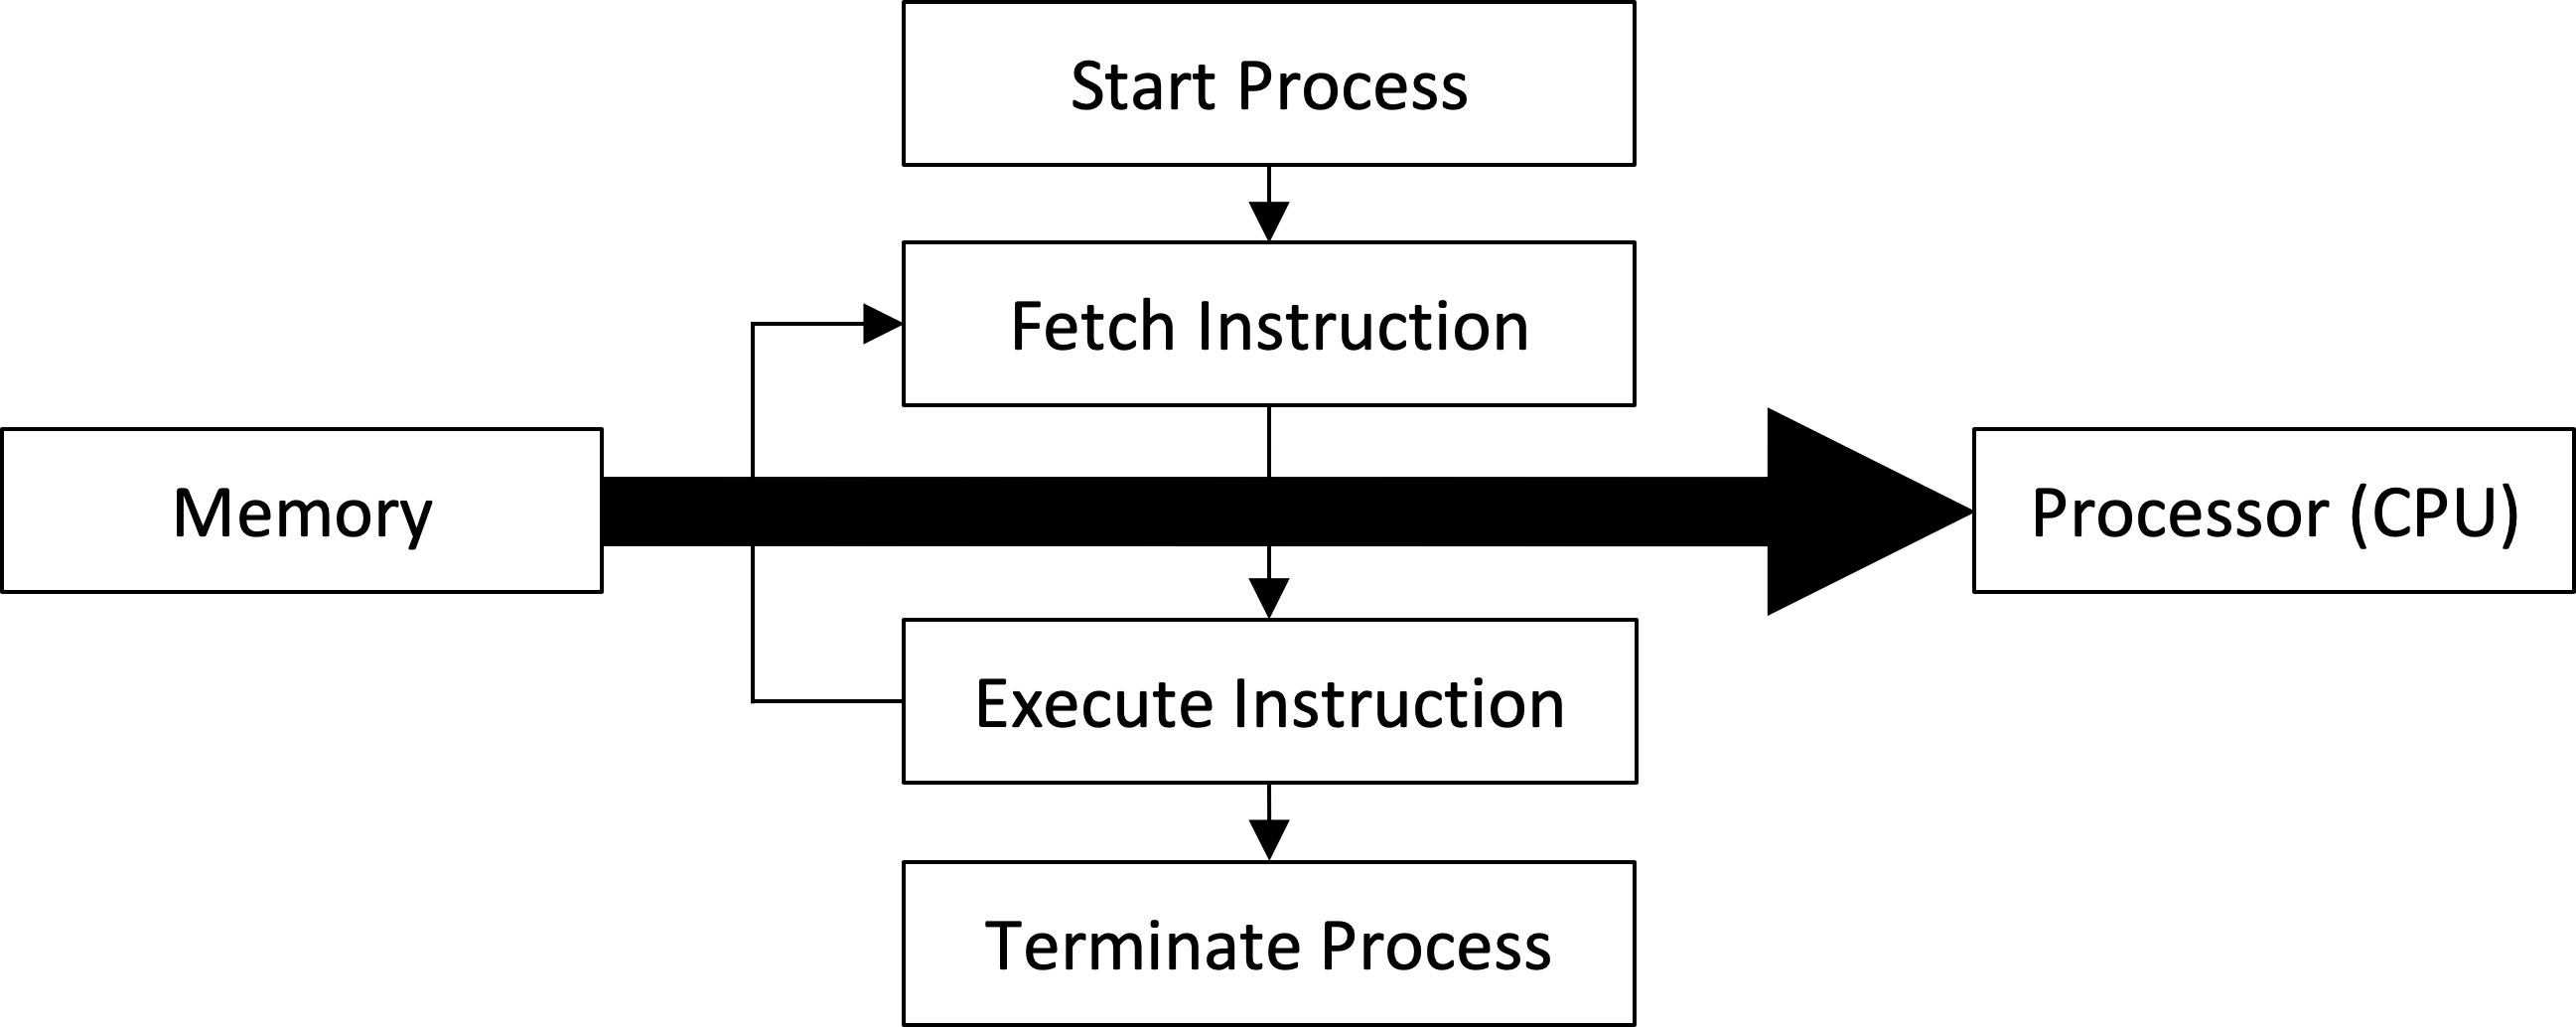
\includegraphics[max size={\textwidth}{\textheight}]{images/chapter-2/simple-fetch-execute-cycle.png}
  \end{minipage}}
  \fbox{\begin{minipage}{\dimexpr \textwidth-2\fboxsep-2\fboxrule}
    \abovecaptionskip=0pt
    \caption{Simple fetch-execute cycle}
  \end{minipage}}
\end{figure}

Once a process is started, instructions are fetched from memory and executed using the CPU. This process will continue until the process is terminated.

This predictable cycle is only feasible to an extent as some processes may be slow or blocked and other may require immediate attention and cannot wait for the current process to terminate. For example, if a process blocks the processor (CPU) because it is waiting for an event to occur, such as a printer to finish its job, or if a high-priority process is supposed to execute as soon as possible. In these cases, interrupts are required.


\section*{Interrupts}

\subsection*{Definition}

An \textbf{interrupt} is a signal sent to the processor indicating that an event caused by hardware or software requires immediate attention.


\subsection*{Types of interrupts}

\begin{longtabu} to \textwidth { X[1.5,l] X[0.2,l] X[7,l]}
	\textbf{\textbullet Input/output (I/O) interrupt}
	& -- &
	Caused by an input/output (I/O) device to signal completion or an error.
	\\
	\\
	\textbf{\textbullet Timer interrupt}
	& -- &
	Caused by a processor timer and is used to alert the operating system (OS) at specific instants.
	\\
	\\
	\textbf{\textbullet Program interrupt}
	& -- &
	Caused by error conditions within user programs or fatal errors.
\end{longtabu}


\subsection*{When do interrupts occur?}

\begin{figure}[H]
  \lineskip=-\fboxrule
  \fbox{\begin{minipage}{\dimexpr \textwidth-2\fboxsep-2\fboxrule}
    \centering
    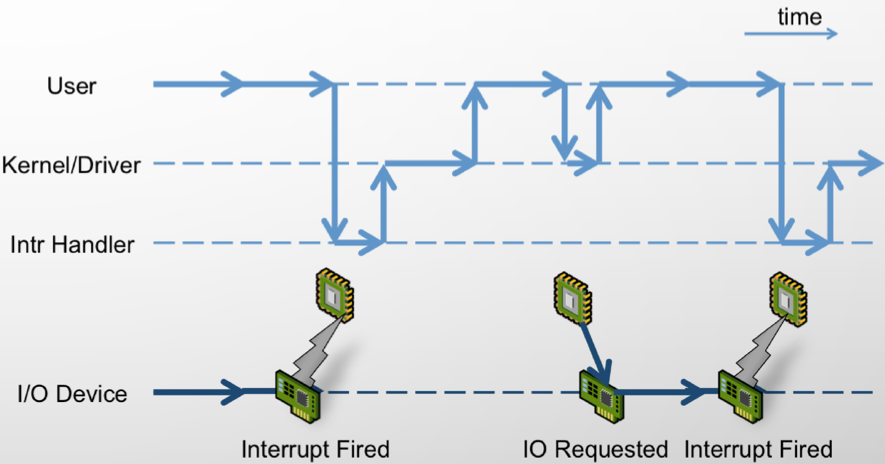
\includegraphics[max size={\textwidth}{\textheight}]{images/chapter-2/interrupt-graph.png}
  \end{minipage}}
  \fbox{\begin{minipage}{\dimexpr \textwidth-2\fboxsep-2\fboxrule}
    \centering
	A process requiring immediate attention is waiting for the processor (CPU).
	
	For example, an input/output (I/O) event occurs.
	
	$\downarrow$
	
	The currently running process’ execution is suspended.
	
	$\downarrow$
	
	Processor switches execution to another process.
	
	$\downarrow$
	
	When input/output (I/O) completes, an interrupt will occur.
	
	$\downarrow$
	
	The execution is diverted to the interrupt handling routine.
	
	An interrupt handling routine (ISR) contains the operations that are performed to deal with an interrupt. Different types of interrupts can have different routines.
	
	$\downarrow$
	
	The suspended program may restart, if conditions are met.
	\end{minipage}}
  \fbox{\begin{minipage}{\dimexpr \textwidth-2\fboxsep-2\fboxrule}
    \abovecaptionskip=0pt
    \caption{Interrupt occurring due to input/output (I/O) event}
  \end{minipage}}
\end{figure}

Interrupts enable operating systems (OSs) to oversee several programs and input/output (I/O) events simultaneously.

This also means that single-core processors can effectively emulate the way in which multi-core processors deal with multiple instructions at a given time by switching between instructions intelligently. Due to the high clock speeds of modern processors, it is easy to give the illusion that true multi-tasking, where two instructions are being processed at once, is taking place on a single-core processor.


\subsection*{Updated fetch-execute cycle}

Given the introduction of interrupts, it is now necessary to update the fetch-execute cycle in order to include the possibility of an interrupt.

\begin{figure}[H]
  \lineskip=-\fboxrule
  \fbox{\begin{minipage}{\dimexpr \textwidth-2\fboxsep-2\fboxrule}
    \centering
    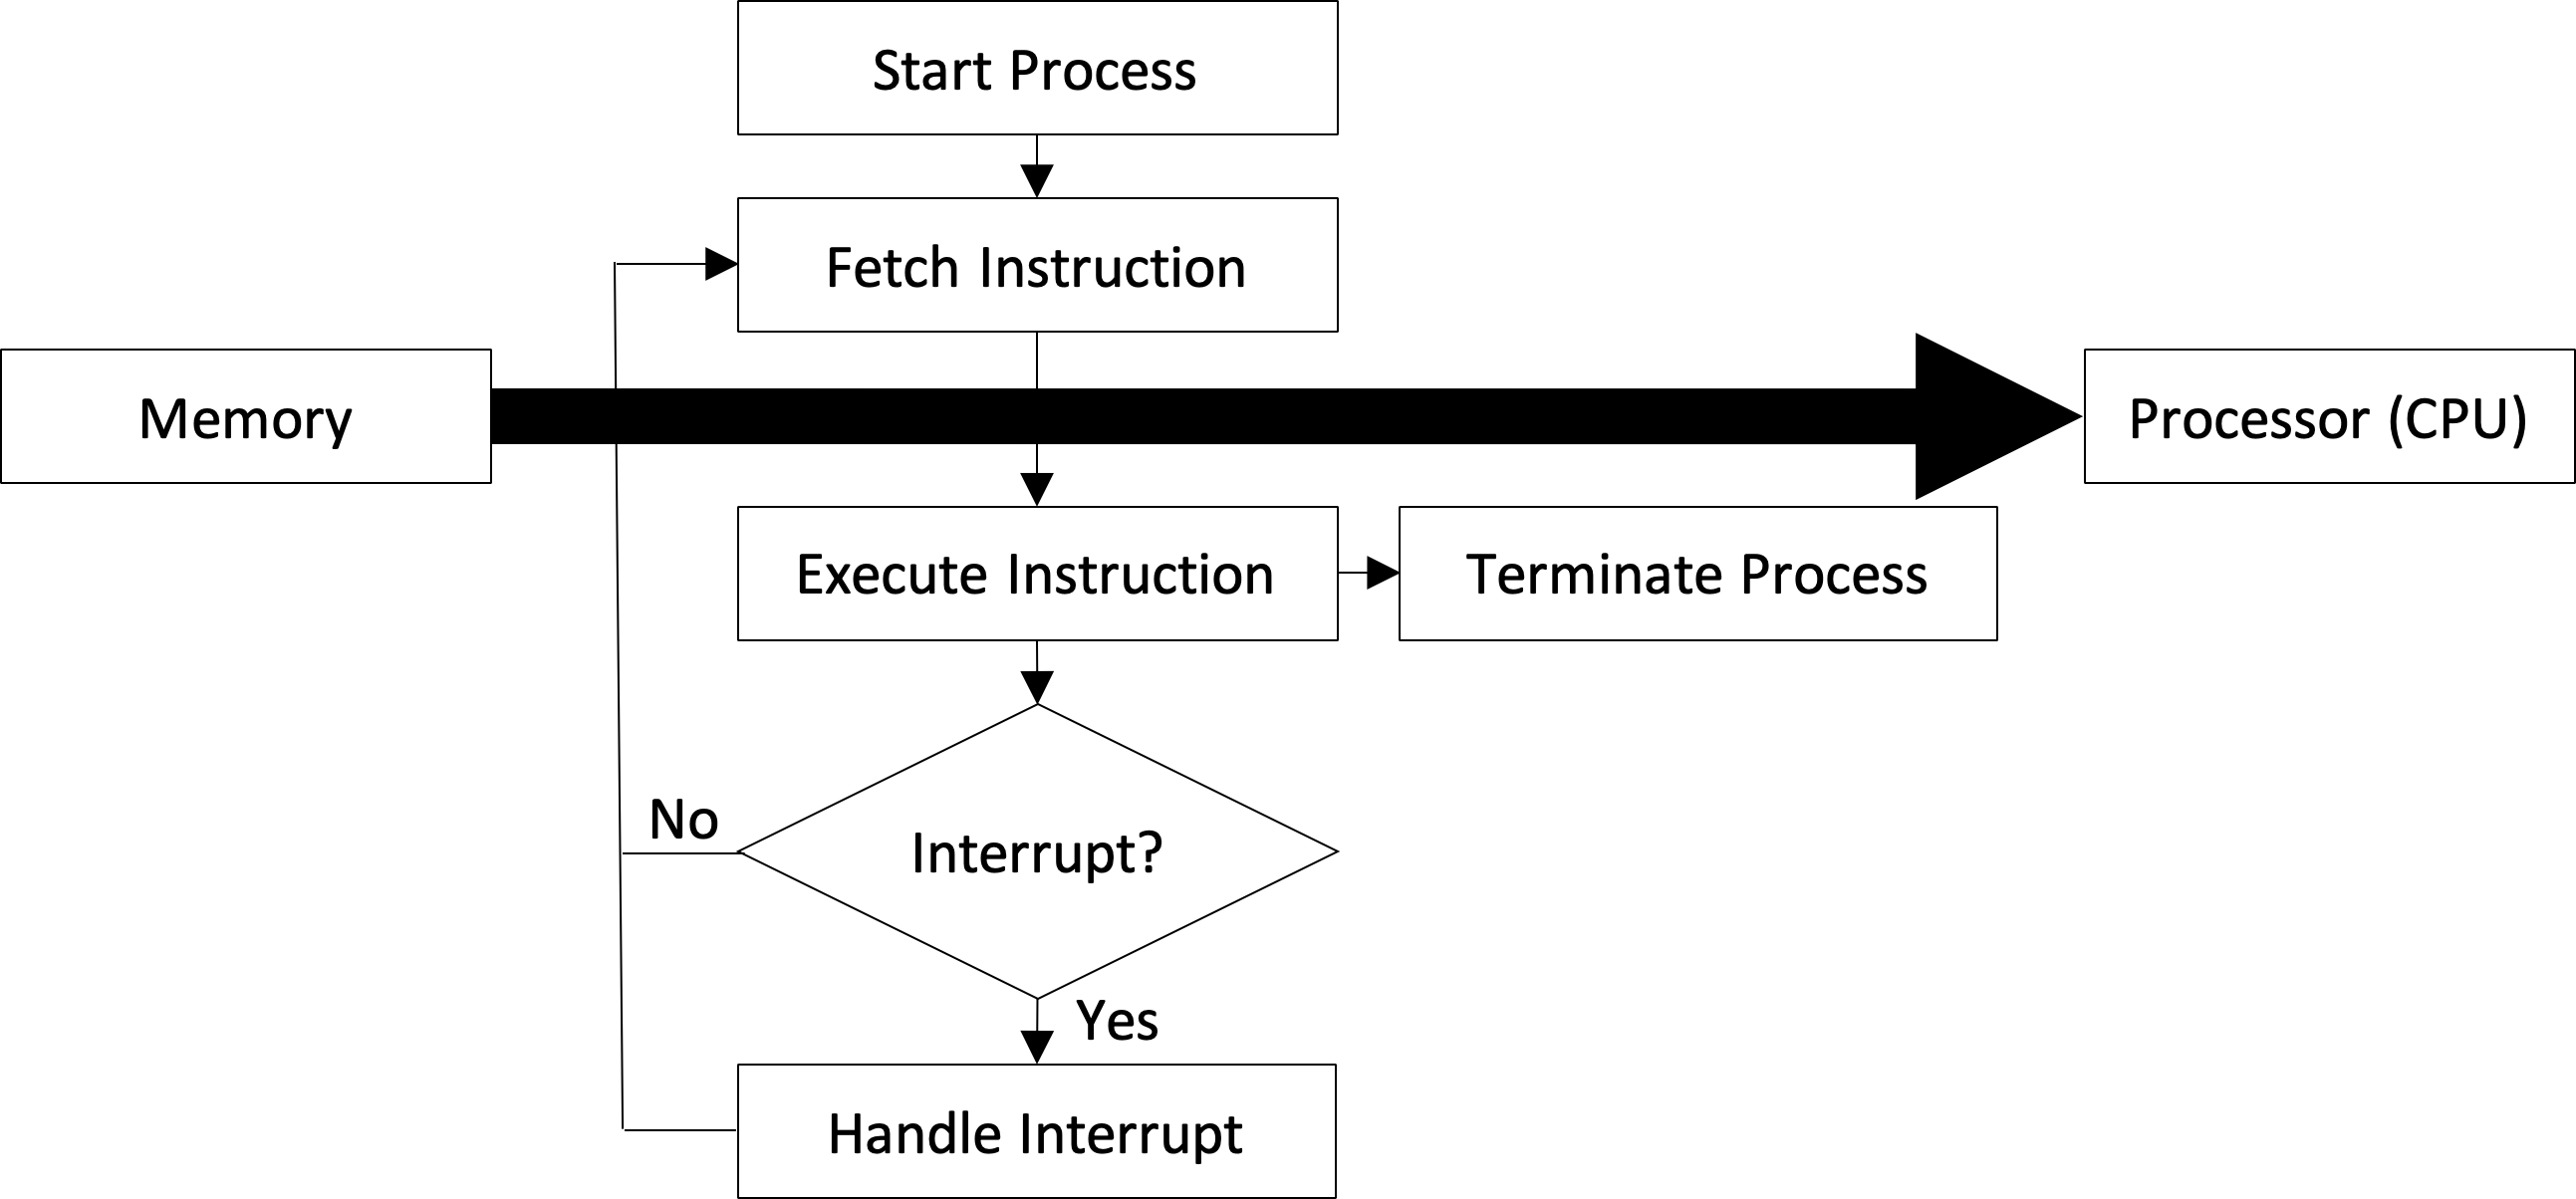
\includegraphics[max size={\textwidth}{\textheight}]{images/chapter-2/updated-fetch-execute-cycle.png}
  \end{minipage}}
  \fbox{\begin{minipage}{\dimexpr \textwidth-2\fboxsep-2\fboxrule}
    \abovecaptionskip=0pt
    \caption{Updated fetch-execute cycle}
  \end{minipage}}
\end{figure}


\section{Concurrency}

\section*{Definition}

\textbf{Concurrency} describes the ability for a program to be decomposed in to parts that can run independently of each other. This means that tasks can be executed out of order and the result would still be the same as if they are executed in order.


\section*{Why is concurrency required}

Concurrency allows the processor (CPU) to run several processes. An example of this is shown by an interrupt occurring due to an input/output (I/O) event occurring (page 24).


\section*{Interleaving}

Concurrency is able to achieve multitasking, that does not require parallel execution, by performing interleaved execution.


\begin{figure}[H]
  \lineskip=-\fboxrule
  \fbox{\begin{minipage}{0.4935\dimexpr \textwidth-2\fboxsep-2\fboxrule}
  	\centering
  	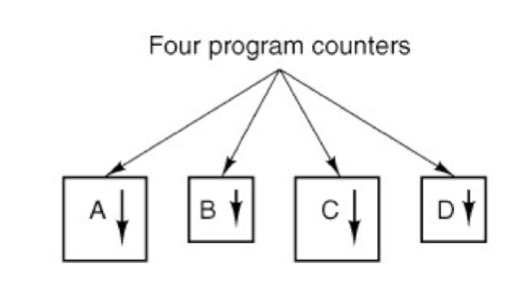
\includegraphics[max size={\textwidth}{\textheight}]{images/chapter-2/interleaving-program-counters.png}
  \end{minipage}
  \begin{minipage}{0.5\dimexpr \textwidth-2\fboxsep-2\fboxrule}
  	\centering
  	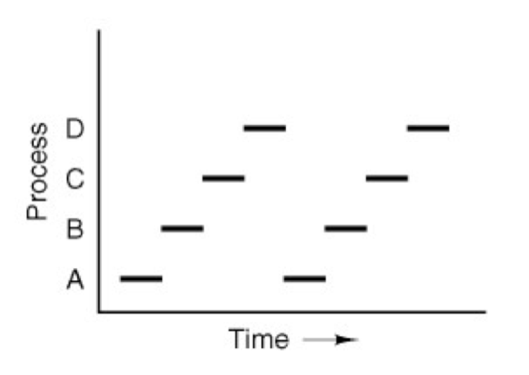
\includegraphics[max size={\textwidth}{\textheight}]{images/chapter-2/interleaving-graph.png}
  \end{minipage}}
  \fbox{\begin{minipage}{\dimexpr \textwidth-2\fboxsep-2\fboxrule}
    \abovecaptionskip=0pt
    \caption{Interleaving}
  \end{minipage}}
\end{figure}


\section{Process scheduling}

\section*{The scheduler}

\subsection*{Definition}

A \textbf{scheduler} uses a scheduling algorithm to determine how to share processor time.


\subsection*{How it works}

After an input/output (I/O) system call or interrupt handling, control is passed to the scheduler to decide which process to execute next.

\begin{figure}[H]
  \lineskip=-\fboxrule
  \fbox{\begin{minipage}{\dimexpr \textwidth-2\fboxsep-2\fboxrule}
    \centering
    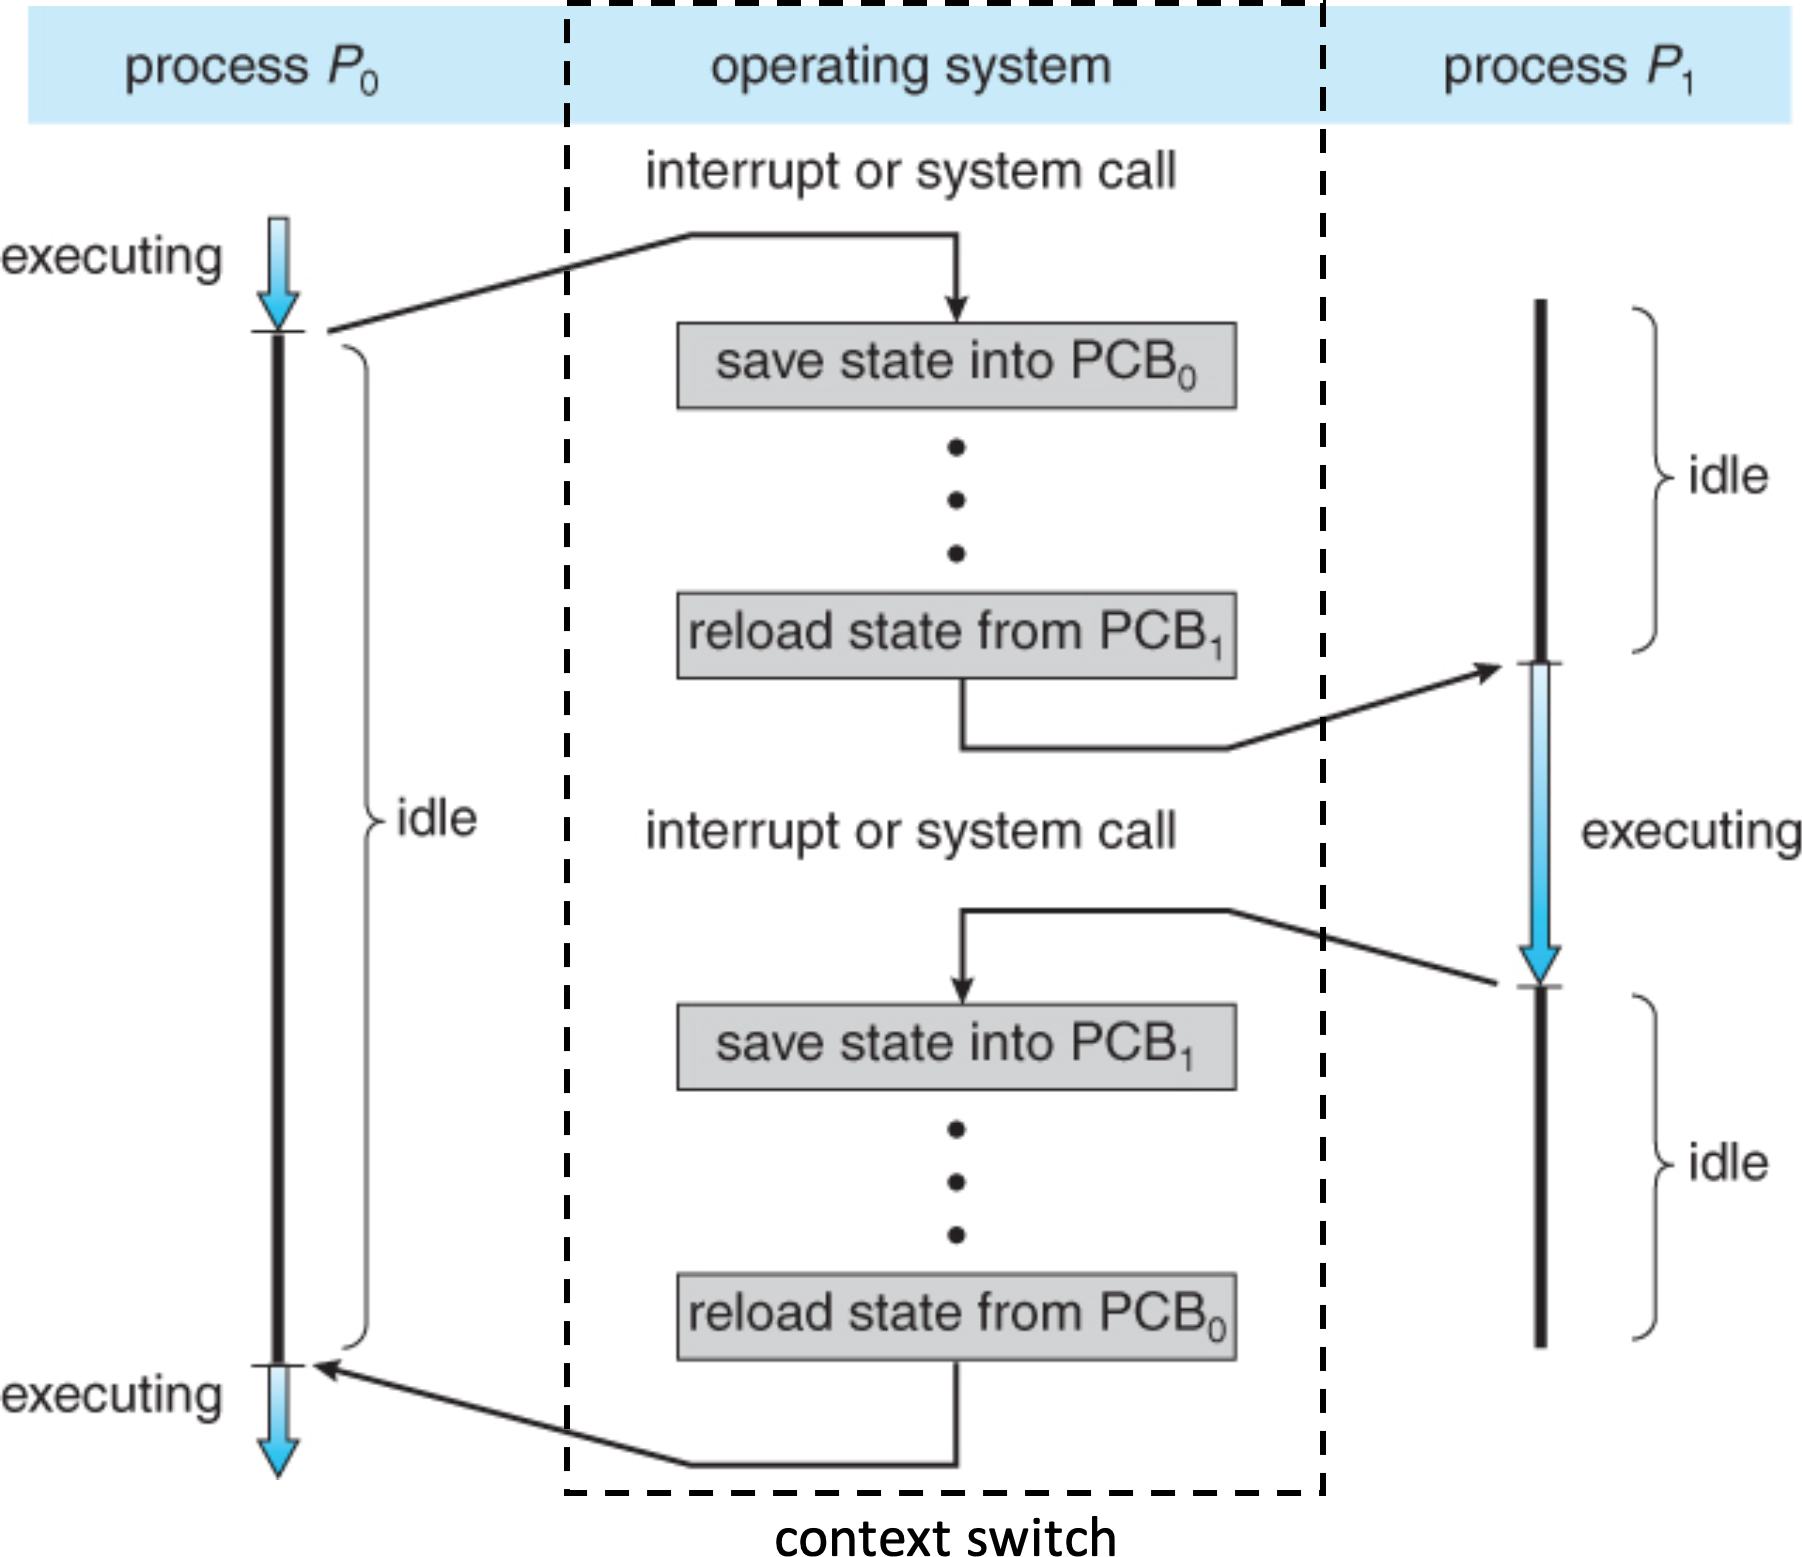
\includegraphics[max size={\textwidth}{\textheight}]{images/chapter-2/the-scheduler.png}
  \end{minipage}}
  \fbox{\begin{minipage}{\dimexpr \textwidth-2\fboxsep-2\fboxrule}
    \abovecaptionskip=0pt
    \caption{The scheduler}
  \end{minipage}}
\end{figure}

The scheduler checks if the current process is still the most suitable to run at this moment in time. If it is control is returned to the process, otherwise:
\begin{itemize}
	\item the state of the current process is saved in the process control block (PCB);
	\item the state of the most suitable process is retrieved from the process control block (PCB); and
	\item control is transferred to the newly selected process at the point indicated by the restored program counter (PC).
\end{itemize}

The action of storing the state of the current process and activating another process is called a context switch.

Context switching must be minimised to reduce overheads created by copying the state of processed and the time taken to perform the switch. However, it is still regarded as important to context switch when appropriate to avoid longer waiting times in the event of a blocked process.


\section*{Scheduling}

\subsection*{Definition}

\textbf{Scheduling} is the act of determining the optimal sequence and timing of assigning execution to processes.


\subsection*{Scheduling criteria}

Different scheduling criteria may be selected depending on the use case for a given computer system.

\begin{longtabu} to \textwidth { X[1.5,l] X[0.2,l] X[7,l]}
	\textbf{\textbullet CPU utilisation}
	& -- &
	Aims to keep the CPU as busy as possible.
	\\
	\\
	\textbf{\textbullet Efficiency}
	& -- &
	Aims to maximise system throughput.
	\\
	\\
	\textbf{\textbullet Fairness}
	& -- &
	Aims to be fair to all running processes or to all users on a multi-user operating system (OS).
\end{longtabu}

This means that different policies and algorithms for scheduling will exist to match these criteria.


\section*{Scheduling policies}

A \textbf{non-preemptive scheduling policy} is one that allows processes to run until complete or incurring an input/output (I/O) wait. These scheduling policies can be described as passive.

A \textbf{preemptive scheduling policy} is one that allows processes to be interrupted and replaced by other processes, generally through timer interrupts.


\section*{Scheduling algorithms}

\subsection*{Definitions}

\textbf{Arrival time} is the instant at which a process is first created.

\textbf{Service time} is the time that it takes for a process to complete if it is in continuous execution.

The \textbf{waiting time} for a process is the sum of time spent in the ready queue during the life of the process. This does not include time that the process is blocked or waiting for input/output (I/O).

In order for a scheduling algorithm to be deemed as fair to all processes, the ratio between waiting time and run time should be about the same for each process.


\subsection*{Case study}

\begin{figure}[H]
  \lineskip=-\fboxrule
  \fbox{\begin{minipage}{\dimexpr \textwidth-2\fboxsep-2\fboxrule}
    \begin{longtabu} to \textwidth {|X[1,c]|X[1,c]|X[1,c]|}
	    \hline
	    \textbf{Process} & \textbf{Arrival Time} & \textbf{Service Time}
	    \\ \hline
	    A & 0 & 3
	    \\ \hline
	    B & 2 & 6
	    \\ \hline
	    C & 4 & 4
	    \\ \hline
	    D & 6 & 5
	    \\ \hline
	    E & 8 & 2
		\\ \hline
	\end{longtabu}
  \end{minipage}}
  \fbox{\begin{minipage}{\dimexpr \textwidth-2\fboxsep-2\fboxrule}
    \abovecaptionskip=0pt
    \caption{Case study}
  \end{minipage}}
\end{figure}

The case study shows different processes (A-E) that all have different arrival times and different service times.

The following examples of scheduling algorithms will refer to this case study to demonstrate their function.


\subsection*{First come, first served (FCFS) / First in, first out (FIFO) – Non-preemptive}

In this algorithm, the first process to arrive is assigned to the processor (CPU) until it is finished. Meanwhile, any other processes that come along are queued up waiting to be processed.

\begin{figure}[H]
  \lineskip=-\fboxrule
  \fbox{\begin{minipage}{0.2935\dimexpr \textwidth-2\fboxsep-2\fboxrule}
  	\centering
  	\begin{longtabu} to \textwidth {|X[1,c]|X[1,c]|X[1,c]|}
	    \hline
	    \textbf{Process} & \textbf{Arrival Time} & \textbf{Service Time}
	    \\ \hline
	    A & 0 & 3
	    \\ \hline
	    B & 2 & 6
	    \\ \hline
	    C & 4 & 4
	    \\ \hline
	    D & 6 & 5
	    \\ \hline
	    E & 8 & 2
		\\ \hline
	\end{longtabu}
  \end{minipage}
  \begin{minipage}{0.7\dimexpr \textwidth-2\fboxsep-2\fboxrule}
  	\centering
  	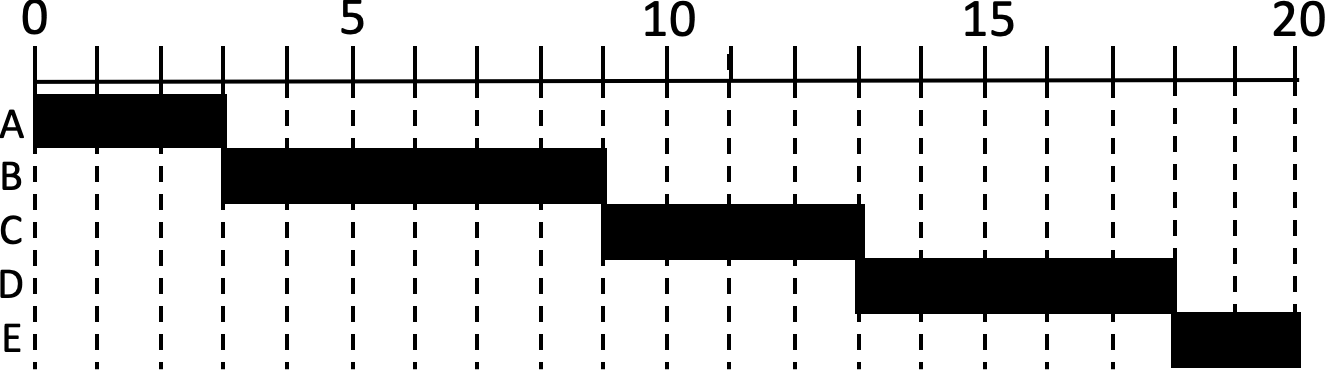
\includegraphics[max size={\textwidth}{\textheight}]{images/chapter-2/temporal-diagram-fcfs.png}
  \end{minipage}}
  \fbox{\begin{minipage}{\dimexpr \textwidth-2\fboxsep-2\fboxrule}
    \abovecaptionskip=0pt
    \caption{Temporal diagram for FCFS / FIFO}
  \end{minipage}}
\end{figure}

\begin{longtabu} to \textwidth {|X[1,l]|X[1,l]|}
    \hline
    \textbf{Advantages} & \textbf{Disadvantages}
    \\ \hline
    \textbf{Simple to implement}.
    &
    \textbf{Does not consider the priority of a process} and therefore the important processes may not be completed quickly.
    \\ \hline
    &
    \textbf{Prevents other processes from starting} while another is in progress and therefore, if processes are of varying sizes, there may be inefficiencies since a single process may take a long time to complete therefore leaving the user waiting before they can perform any other actions.
	\\ \hline
	\multicolumn{2}{|p{\textwidth}|}{\textbf{Favours long processes} as all processes are given the opportunity to run until completion and therefore, some shorter processes may not be able to start processing until the longer processes are finished.}
	\\ \hline
\end{longtabu}
	

\subsection*{Shortest job first (SJF) – Non-preemptive}

In this algorithm, the process with the shortest estimated run time is assigned to the processor (CPU) until it is finished. Meanwhile, any other processes that come along are queued up waiting to be processed.

\begin{figure}[H]
  \lineskip=-\fboxrule
  \fbox{\begin{minipage}{0.2935\dimexpr \textwidth-2\fboxsep-2\fboxrule}
  	\centering
  	\begin{longtabu} to \textwidth {|X[1,c]|X[1,c]|X[1,c]|}
	    \hline
	    \textbf{Process} & \textbf{Arrival Time} & \textbf{Service Time}
	    \\ \hline
	    A & 0 & 3
	    \\ \hline
	    B & 2 & 6
	    \\ \hline
	    C & 4 & 4
	    \\ \hline
	    D & 6 & 5
	    \\ \hline
	    E & 8 & 2
		\\ \hline
	\end{longtabu}
  \end{minipage}
  \begin{minipage}{0.7\dimexpr \textwidth-2\fboxsep-2\fboxrule}
  	\centering
  	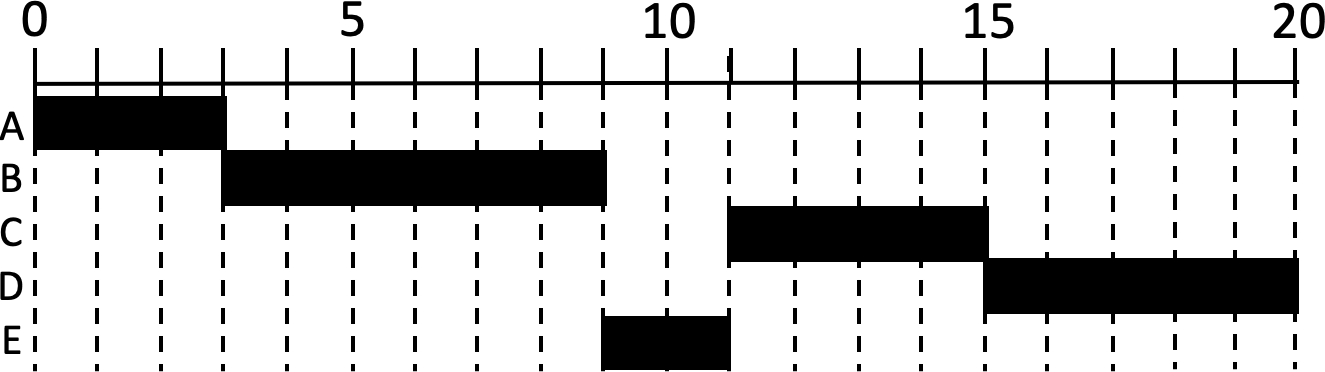
\includegraphics[max size={\textwidth}{\textheight}]{images/chapter-2/temporal-diagram-sjf.png}
  \end{minipage}}
  \fbox{\begin{minipage}{\dimexpr \textwidth-2\fboxsep-2\fboxrule}
    \abovecaptionskip=0pt
    \caption{Temporal diagram for SJF}
  \end{minipage}}
\end{figure}

\begin{longtabu} to \textwidth {|X[1,l]|X[1,l]|}
    \hline
    \textbf{Advantages} & \textbf{Disadvantages}
    \\ \hline
    \textbf{Simple to implement}.
    &
    \textbf{Does not consider the priority of a process} and therefore the important processes may not be completed quickly.
    \\ \hline
  	\textbf{Shorter processes are processed quickly} because they take precedence.
    &
    \textbf{Relies on an estimation} of how long a process will take which could be incorrect.
    \\ \hline
  	\textbf{Minimises the average time taken to complete a process} because the shortest processes take precedence.
    &
    \textbf{Prevents other processes from starting} while another is in progress and therefore, if processes are of varying sizes, there may be inefficiencies since a single process may take a long time to complete therefore leaving the user waiting before they can perform any other actions.
	\\ \hline
	\multicolumn{2}{|p{\textwidth}|}{\textbf{Favours long processes} as the processes with the shortest estimated time are given the opportunity to run until completion and therefore, some longer processes may not be able to start processing until there are no more shorter processes currently running or ready to be processed.}
	\\ \hline
\end{longtabu}


\subsection*{Shortest remaining time (SRT) – Preemptive}

In this algorithm, the process with the shortest estimated remaining time is assigned to the processor (CPU). If a process becomes ready that has a shorter remaining time, it will be pre-empted to allow the new process to start and the scheduler is switched to that new process.

\begin{figure}[H]
  \lineskip=-\fboxrule
  \fbox{\begin{minipage}{0.2935\dimexpr \textwidth-2\fboxsep-2\fboxrule}
  	\centering
  	\begin{longtabu} to \textwidth {|X[1,c]|X[1,c]|X[1,c]|}
	    \hline
	    \textbf{Process} & \textbf{Arrival Time} & \textbf{Service Time}
	    \\ \hline
	    A & 0 & 3
	    \\ \hline
	    B & 2 & 6
	    \\ \hline
	    C & 4 & 4
	    \\ \hline
	    D & 6 & 5
	    \\ \hline
	    E & 8 & 2
		\\ \hline
	\end{longtabu}
  \end{minipage}
  \begin{minipage}{0.7\dimexpr \textwidth-2\fboxsep-2\fboxrule}
  	\centering
  	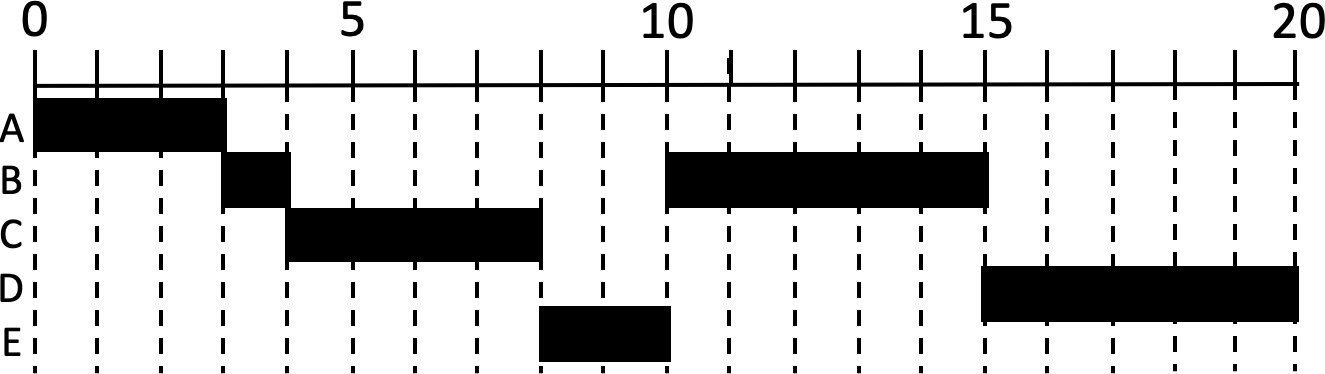
\includegraphics[max size={\textwidth}{\textheight}]{images/chapter-2/temporal-diagram-srt.png}
  \end{minipage}}
  \fbox{\begin{minipage}{\dimexpr \textwidth-2\fboxsep-2\fboxrule}
    \abovecaptionskip=0pt
    \caption{Temporal diagram for SRT}
  \end{minipage}}
\end{figure}

\begin{longtabu} to \textwidth {|X[1,l]|X[1,l]|}
    \hline
    \textbf{Advantages} & \textbf{Disadvantages}
    \\ \hline
    \textbf{High throughput} because the number of processes completed is high due to the shortest processes taking precedence.
    &
    \textbf{Does not consider the priority of a process} and therefore the important processes may not be completed quickly.
    \\ \hline
  	\textbf{Shorter processes are processed quickly} because they take precedence.
    &
    \textbf{Relies on an estimation} of how long a process will take which could be incorrect.
    \\ \hline
  	
    &
    \textbf{Can be inefficient} if a large process is in progress and shorter processes are being added to the queue because they will take precedence.
	\\ \hline
	\multicolumn{2}{|p{\textwidth}|}{\textbf{Favours long processes} as the processes with the shortest estimated time are given the opportunity to run until a process with a shorter estimated time is ready and therefore, some longer processes may not be able to start processing until there are no more shorter processes currently running or ready to be processed.}
	\\ \hline
\end{longtabu}


\subsection*{Highest response ratio next (HRRN) – Preemptive}

In this algorithm, the process with the highest priority is assigned to the processor (CPU). If a process becomes ready that has a higher priority, it will be pre-empted to allow the new process to start and the scheduler is switched to that new process.

The priority of a process may be based on memory, time and/or any other resource requirement such as:
\[\frac{waiting time + run time}{run time}\]

\begin{figure}[H]
  \lineskip=-\fboxrule
  \fbox{\begin{minipage}{0.2935\dimexpr \textwidth-2\fboxsep-2\fboxrule}
  	\centering
  	\begin{longtabu} to \textwidth {|X[1,c]|X[1,c]|X[1,c]|}
	    \hline
	    \textbf{Process} & \textbf{Arrival Time} & \textbf{Service Time}
	    \\ \hline
	    A & 0 & 3
	    \\ \hline
	    B & 2 & 6
	    \\ \hline
	    C & 4 & 4
	    \\ \hline
	    D & 6 & 5
	    \\ \hline
	    E & 8 & 2
		\\ \hline
	\end{longtabu}
  \end{minipage}
  \begin{minipage}{0.7\dimexpr \textwidth-2\fboxsep-2\fboxrule}
  	\centering
  	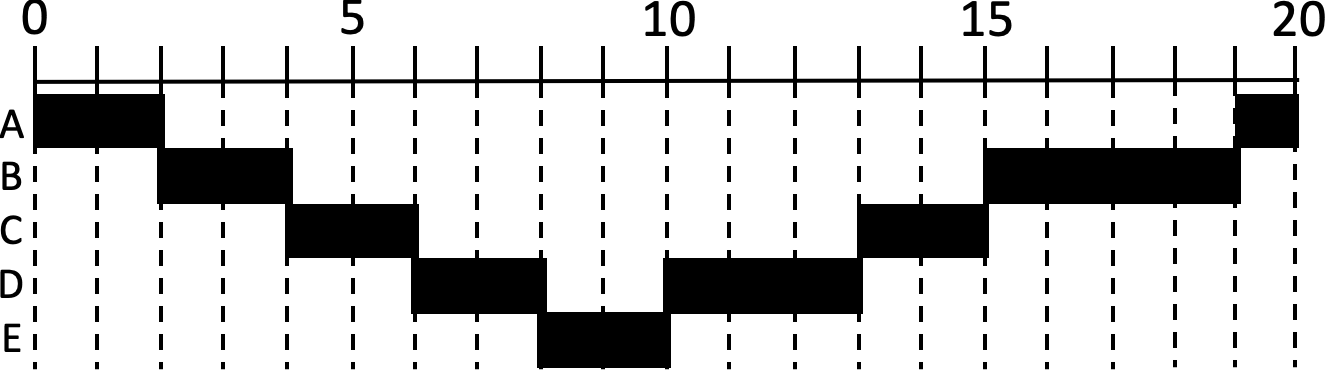
\includegraphics[max size={\textwidth}{\textheight}]{images/chapter-2/temporal-diagram-hrrn.png}
  	This diagram assumes that the processes are assigned a letter in reverse order of priority, such that E has the greatest priority and A has the lowest priority.
  \end{minipage}}
  \fbox{\begin{minipage}{\dimexpr \textwidth-2\fboxsep-2\fboxrule}
    \abovecaptionskip=0pt
    \caption{Temporal diagram for HRRN}
  \end{minipage}}
\end{figure}

\begin{longtabu} to \textwidth {|X[1,l]|X[1,l]|}
    \hline
    \textbf{Advantages} & \textbf{Disadvantages}
    \\ \hline
    \textbf{High throughput} because the number of processes completed is high due to the shortest processes taking precedence.
    &
    \textbf{Does not consider the priority of a process} and therefore the important processes may not be completed quickly.
    \\ \hline
  	\textbf{Shorter processes are processed quickly} because they take precedence.
    &
    \textbf{Relies on an estimation} of how long a process will take which could be incorrect.
    \\ \hline
  	
    &
    \textbf{Can be inefficient} if a large process is in progress and shorter processes are being added to the queue because they will take precedence.
	\\ \hline
\end{longtabu}


\subsection*{Round robin (RR) – Preemptive}

In this algorithm, each process is dispatched to the processor (CPU) on a “first in, first out” (FIFO) basis with a fixed time quantum.

Each time quantum is typically 10-20ms. Modern processor (CPU) clock frequencies are typically greater than 2GHz, which implies clock periods of 5×10$^{-7}$ms. This shows that the given time quantum is relatively large compared to a typically processor’s (CPU’s) clock period.

If a process experiences a timeout, this will mean that it has run over its fixed time quantum. In which case, the process will be interrupted and returned to the back of the queue.

A system designer may wish to choose a time quantum that is most appropriate for a given system. This may be done by measuring the average service time and waiting time for the processes that will be running on the system and design the fixed time quantum around these figures. It may be that a system designer wishes to minimise the number of processes that are interrupted by another process.

\begin{figure}[H]
  \lineskip=-\fboxrule
  \fbox{\begin{minipage}{\dimexpr \textwidth-2\fboxsep-2\fboxrule}
    \centering
    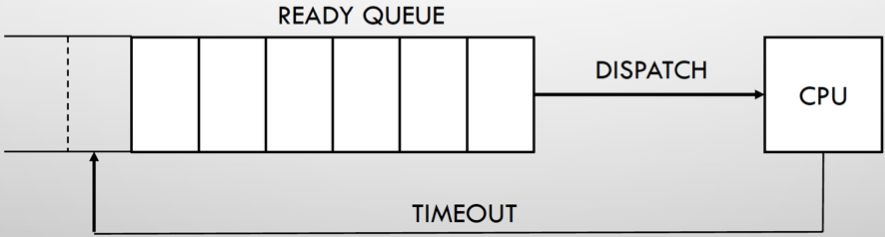
\includegraphics[max size={\textwidth}{\textheight}]{images/chapter-2/round-robin.png}
  \end{minipage}}
  \fbox{\begin{minipage}{\dimexpr \textwidth-2\fboxsep-2\fboxrule}
    \abovecaptionskip=0pt
    \caption{RR}
  \end{minipage}}
\end{figure}

\begin{figure}[H]
  \lineskip=-\fboxrule
  \fbox{\begin{minipage}{0.2935\dimexpr \textwidth-2\fboxsep-2\fboxrule}
  	\centering
  	\begin{longtabu} to \textwidth {|X[1,c]|X[1,c]|X[1,c]|}
	    \hline
	    \textbf{Process} & \textbf{Arrival Time} & \textbf{Service Time}
	    \\ \hline
	    A & 0 & 3
	    \\ \hline
	    B & 2 & 6
	    \\ \hline
	    C & 4 & 4
	    \\ \hline
	    D & 6 & 5
	    \\ \hline
	    E & 8 & 2
		\\ \hline
	\end{longtabu}
  \end{minipage}
  \begin{minipage}{0.7\dimexpr \textwidth-2\fboxsep-2\fboxrule}
  	\centering
  	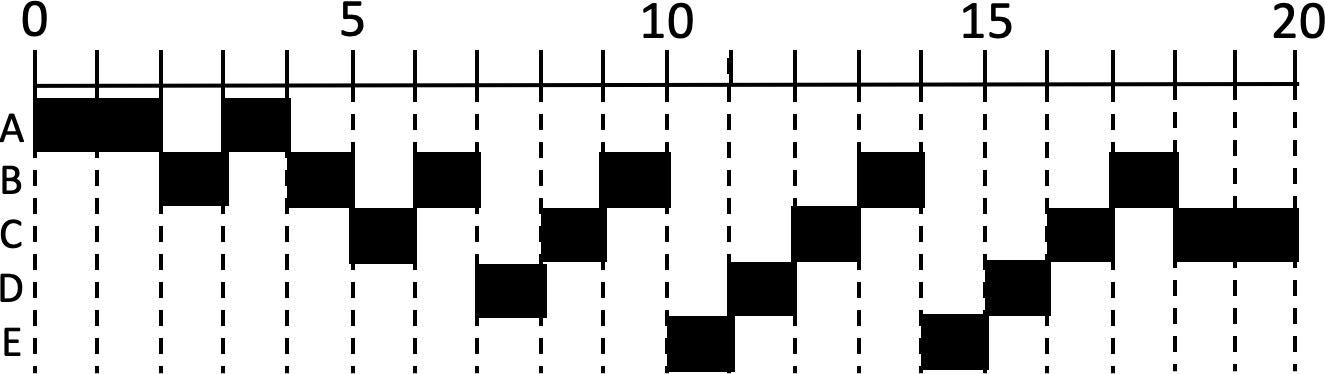
\includegraphics[max size={\textwidth}{\textheight}]{images/chapter-2/temporal-diagram-rr-1.png}
  \end{minipage}}
  \fbox{\begin{minipage}{\dimexpr \textwidth-2\fboxsep-2\fboxrule}
    \abovecaptionskip=0pt
    \caption{Temporal diagram for RR with a fixed time quantum of 1 (q = 1)}
  \end{minipage}}
\end{figure}

\begin{figure}[H]
  \lineskip=-\fboxrule
  \fbox{\begin{minipage}{0.2935\dimexpr \textwidth-2\fboxsep-2\fboxrule}
  	\centering
  	\begin{longtabu} to \textwidth {|X[1,c]|X[1,c]|X[1,c]|}
	    \hline
	    \textbf{Process} & \textbf{Arrival Time} & \textbf{Service Time}
	    \\ \hline
	    A & 0 & 3
	    \\ \hline
	    B & 2 & 6
	    \\ \hline
	    C & 4 & 4
	    \\ \hline
	    D & 6 & 5
	    \\ \hline
	    E & 8 & 2
		\\ \hline
	\end{longtabu}
  \end{minipage}
  \begin{minipage}{0.7\dimexpr \textwidth-2\fboxsep-2\fboxrule}
  	\centering
  	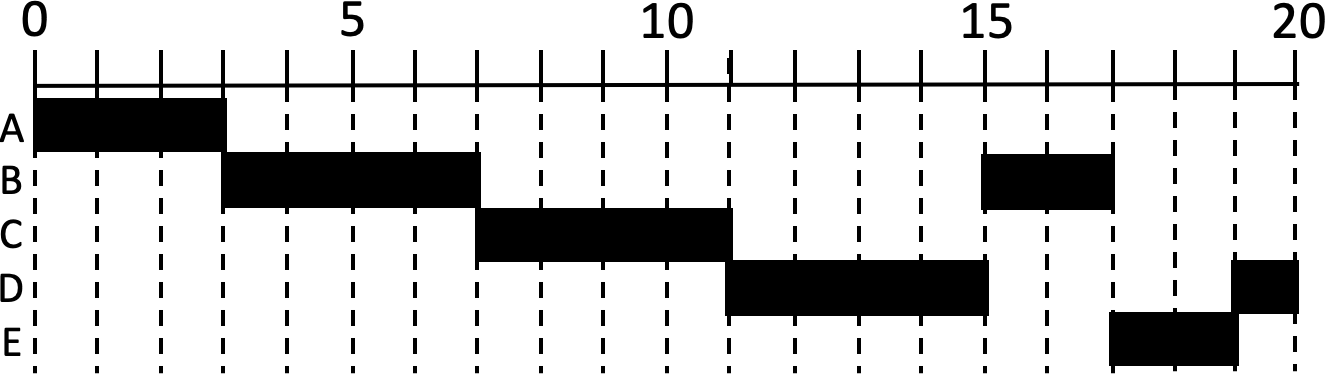
\includegraphics[max size={\textwidth}{\textheight}]{images/chapter-2/temporal-diagram-rr-4.png}
  \end{minipage}}
  \fbox{\begin{minipage}{\dimexpr \textwidth-2\fboxsep-2\fboxrule}
    \abovecaptionskip=0pt
    \caption{Temporal diagram for RR with a fixed time quantum of 4 (q = 4)}
  \end{minipage}}
\end{figure}

\begin{longtabu} to \textwidth {|X[1,l]|X[1,l]|}
    \hline
    \textbf{Advantages} & \textbf{Disadvantages}
    \\ \hline
    \textbf{Simple to implement}.
    &
    \textbf{Heavy overhead} due to continuous context switches.
    \\ \hline
  	\textbf{Suitable for some types of computer systems}, such as those which will be running processes of similar priority and size.
    &
    \textbf{Does not consider the priority of a process} and therefore the important processes may not be completed quickly.
    \\ \hline
    &
    \textbf{Does not consider the size of a process} and therefore, if processes are of varying sizes, there may be inefficiencies since a single process may take a long time to complete thus leaving the user waiting before they can perform any other actions.
	\\ \hline
\end{longtabu}


\section*{Multi-level queueing}

\subsection*{Definition}

\textbf{Multi-level queueing} is a queue with a predefined number of levels which consist of several independent queues.


\subsection*{How it works}

Multi-level queueing makes use of other existing scheduling algorithms.

\begin{figure}[H]
  \lineskip=-\fboxrule
  \fbox{\begin{minipage}{\dimexpr \textwidth-2\fboxsep-2\fboxrule}
    \centering
    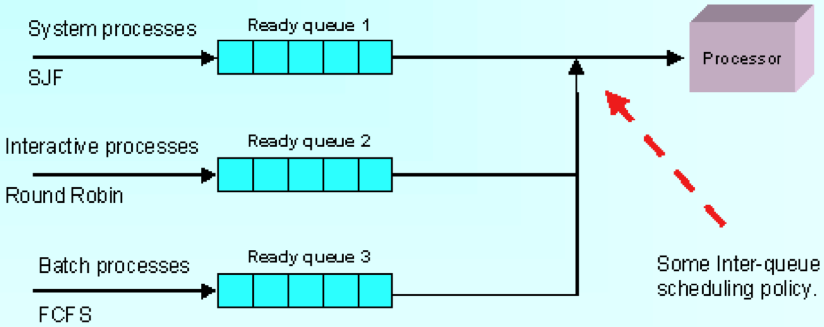
\includegraphics[max size={\textwidth}{\textheight}]{images/chapter-2/multi-level-queueing.png}
  \end{minipage}}
  \fbox{\begin{minipage}{\dimexpr \textwidth-2\fboxsep-2\fboxrule}
    \abovecaptionskip=0pt
    \caption{Multi-level queueing}
  \end{minipage}}
\end{figure}

Each queue has a different priority; the top queue has the highest priority and the bottom queue has the lowest priority. Processes are able to move between queues if their priority changes.

There is some form of inter-queue scheduling policy that governs the assignment of processes from each queue to the processor (CPU).

The queues in a multi-level queueing system may differ between operating system (OS). For example, the scheduler used by the Minix operating system (OS) uses multi-level queueing and implements 16 queues.

\begin{longtabu} to \textwidth {|X[1,l]|X[1,l]|}
    \hline
    \textbf{Advantages} & \textbf{Disadvantages}
    \\ \hline
    \textbf{Allows scheduling optimisation} as a system designer may be able to leverage the advantages of a range of different scheduling algorithms.
    &
    \\ \hline
  	\textbf{Maintains common processes} as it is possible to split processes in to different queues depending on their nature. For example, input/output processes could be in one queue while processor (CPU) processes are in another queue.
    &
    \\ \hline
    \textbf{Helps to prevent bottlenecks} because input/output (I/O) devices are slower than the processor speed and therefore maximising processes involving input/output (I/O) devices ensures that these devices are continuously busy.
    &
	\\ \hline
\end{longtabu}


\chapter{Threads and Concurrency}

\section{What are threads?}

\section*{Definition}

A \textbf{thread} is an independent path/sequence of execution with in a process and can be managed independently by a scheduler. A process many contain many threads.


\section*{Multi-threading}

\subsection*{How it works}

As mentioned in the previous section, a process (or job/task) shows a program in execution and is a particular instance of a program. By default, these processes are run by means of “single execution thread”.

However, different parts of the same process could be parallelised in order to allow multi-threading.

Multi-threading provides a way of improving application performance and therefore improving the efficiency and/or usability of a computer system.

\begin{figure}[H]
  \lineskip=-\fboxrule
  \fbox{\begin{minipage}{\dimexpr \textwidth-2\fboxsep-2\fboxrule}
    \centering
    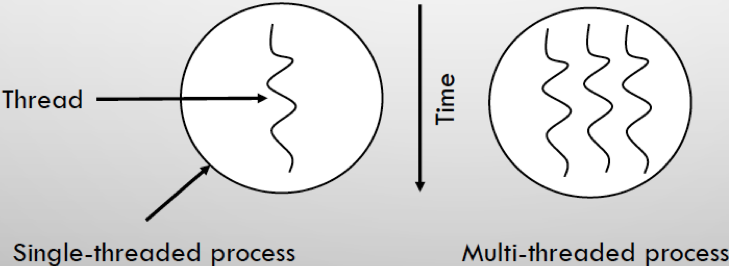
\includegraphics[max size={\textwidth}{\textheight}]{images/chapter-3/single-threaded-vs-multi-threaded.png}
  \end{minipage}}
  \fbox{\begin{minipage}{\dimexpr \textwidth-2\fboxsep-2\fboxrule}
    \abovecaptionskip=0pt
    \caption{Single-threaded vs multi-threaded}
  \end{minipage}}
\end{figure}


\subsection*{Example}

\begin{figure}[H]
  \lineskip=-\fboxrule
  \fbox{\begin{minipage}{0.4935\dimexpr \textwidth-2\fboxsep-2\fboxrule}
  	\centering
  	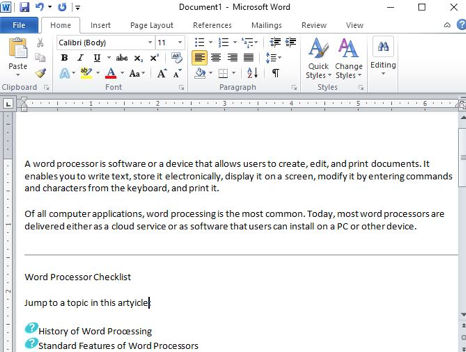
\includegraphics[max size={\textwidth}{\textheight}]{images/chapter-3/microsoft-word.png}
  \end{minipage}
  \begin{minipage}{0.5\dimexpr \textwidth-2\fboxsep-2\fboxrule}
	In this example, a thread could be assigned to each of the following tasks:
	\begin{itemize}
		\item user input, such as keyboard and mouse input;
		\item auto-saving document;
		\item spell-checking document; and
		\item printing in the background.
	\end{itemize}
	This is possible as all of these tasks can be run in parallel as they do not require information from one another.
  \end{minipage}}
  \fbox{\begin{minipage}{\dimexpr \textwidth-2\fboxsep-2\fboxrule}
    \abovecaptionskip=0pt
    \caption{Example of multi-threading in Microsoft Word}
  \end{minipage}}
\end{figure}


\section*{Threads vs processes}

\subsection*{Comparison}

Threads and processes share some similarities however, there are also some distinct differences.

\begin{figure}[H]
  \lineskip=-\fboxrule
  \fbox{\begin{minipage}{\dimexpr \textwidth-2\fboxsep-2\fboxrule}
    \centering
    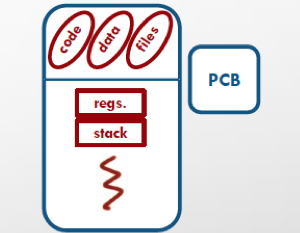
\includegraphics[max size={\textwidth}{\textheight}]{images/chapter-3/single-threaded-process.png}
  \end{minipage}}
  \fbox{\begin{minipage}{\dimexpr \textwidth-2\fboxsep-2\fboxrule}
    \abovecaptionskip=0pt
    \caption{Single-threaded process}
  \end{minipage}}
\end{figure}

\begin{figure}[H]
  \lineskip=-\fboxrule
  \fbox{\begin{minipage}{\dimexpr \textwidth-2\fboxsep-2\fboxrule}
    \centering
    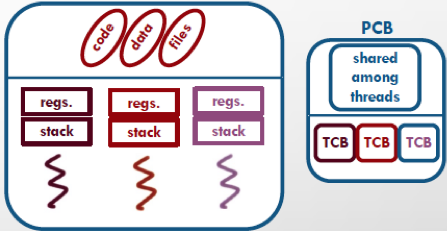
\includegraphics[max size={\textwidth}{\textheight}]{images/chapter-3/multi-threaded-process.png}
  \end{minipage}}
  \fbox{\begin{minipage}{\dimexpr \textwidth-2\fboxsep-2\fboxrule}
    \abovecaptionskip=0pt
    \caption{Multi-threaded process}
  \end{minipage}}
\end{figure}

\begin{figure}[H]
  \lineskip=-\fboxrule
  \fbox{\begin{minipage}{\dimexpr \textwidth-2\fboxsep-2\fboxrule}
    \centering
    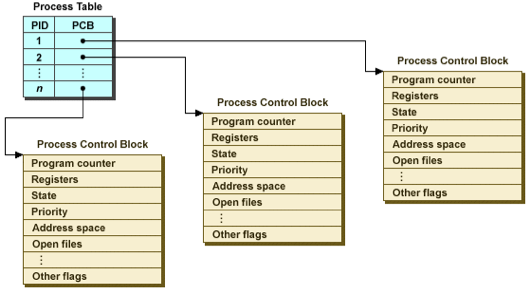
\includegraphics[max size={\textwidth}{\textheight}]{images/chapter-3/process-table-and-control-block.png}
  \end{minipage}}
  \fbox{\begin{minipage}{\dimexpr \textwidth-2\fboxsep-2\fboxrule}
    \abovecaptionskip=0pt
    \caption{Process table and process control blocks}
  \end{minipage}}
\end{figure}

\begin{figure}[H]
  \lineskip=-\fboxrule
  \fbox{\begin{minipage}{\dimexpr \textwidth-2\fboxsep-2\fboxrule}
    \begin{longtabu} to \textwidth {|X[0.8,c]|X[2,l]|X[2,l]|}
	    \hline
	     & \textbf{Threads} & \textbf{Processes}
	    \\ \hline
		\multirow{7}{*}{Similarities}
		& Sequential flow of control with start and end.
		& Sequential flow of control with start and end.
		\\
		\cline{2-3} 
		& At any time, a thread has a single point of execution.
		& At any time, a process has a single point of execution.
		\\
		\cline{2-3} 
		& Has its own execution context, stack (history) and program counter stored in a thread control block (TCB).
		& Has its own execution context, stack (history) and program counter stored in a process control block (PCB).
		\\
		\cline{2-3} 
		& Follows the three-state model in which the thread can be running, blocked or ready.
		& Follows the three-state model in which the process can be running, blocked or ready.
		\\
		\cline{2-3} 
		& Context switching can happen for threads.
		& Context switching can happen for processes.
		\\
		\cline{2-3} 
		& A thread can spawn another thread.
		& A process can spawn another process.
		\\
		\cline{2-3} 
		& A thread is often called a lightweight process. &
		\\ \hline
		\multirow{5}{*}{Differences}
		& A thread cannot exist on its own, instead it exists within a process.
		& A process does not require a parent entity.
		\\
		\cline{2-3} 
		& Usually created and/or controlled by a process.
		& A process is not typically created and/or controlled by another process.
		\\
		\cline{2-3} 
		& Threads can share process properties, including memory and open files.
		& Processes cannot share process properties with other processes.
		\\
		\cline{2-3} 
		& Inexpensive creation and context switching as does not require separate address space.
		& Expensive creation and context switching as requires separate address space.
		\\
		\cline{2-3} 
		& When running multiple threads concurrently, they share an address space.
		& When running multiple processes concurrently, they are resources, such as memory, disk and printers.
		\\ \hline
	\end{longtabu}
  \end{minipage}}
  \fbox{\begin{minipage}{\dimexpr \textwidth-2\fboxsep-2\fboxrule}
    \abovecaptionskip=0pt
    \caption{Threads vs processes}
  \end{minipage}}
\end{figure}


\subsection*{Properties}

\begin{figure}[H]
  \lineskip=-\fboxrule
  \fbox{\begin{minipage}{\dimexpr \textwidth-2\fboxsep-2\fboxrule}
    \begin{longtabu} to \textwidth {|X[1,l]|X[1,l]|}
	    \hline
		\textbf{Per process items}
		& \textbf{Per thread items}
		\\ \hline
		Address space & Program counter
		\\ \hline
		Global variables & Registers
		\\ \hline
		Open files & Stack
		\\ \hline
		Child processes & State
		\\ \hline
		Pending alarms &
		\\ \hline
		Signals and signal handlers &
		\\ \hline
		Accounting information &
		\\ \hline
	\end{longtabu}
  \end{minipage}}
  \fbox{\begin{minipage}{\dimexpr \textwidth-2\fboxsep-2\fboxrule}
    \abovecaptionskip=0pt
    \caption{Threads vs processes}
  \end{minipage}}
\end{figure}

Process properties are shared between threads.
Thread properties are local and private to each thread.


\section{Sequential and concurrent programming}

\section*{Sequential programming}

\subsection*{Definition}

\textbf{Sequential programming} is the traditional activity of constructing a computer program using a sequential programming language.


\subsection*{How it works}

This involves a programming methodology that assumes statements are executed in order/sequence.

Programs written using sequential programming are assumed to execute on a single-CPU system and have a single thread of control.

\begin{figure}[H]
  \lineskip=-\fboxrule
  \fbox{\begin{minipage}{\dimexpr \textwidth-2\fboxsep-2\fboxrule}
    \centering
    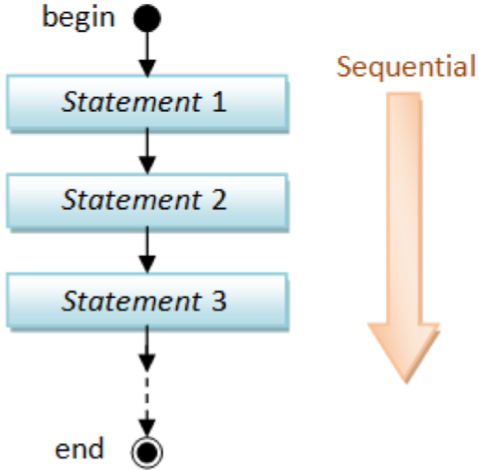
\includegraphics[max size={\textwidth}{\textheight}]{images/chapter-3/sequential-program.png}
  \end{minipage}}
  \fbox{\begin{minipage}{\dimexpr \textwidth-2\fboxsep-2\fboxrule}
    \abovecaptionskip=0pt
    \caption{Sequential program}
  \end{minipage}}
\end{figure}


\subsection*{Evaluation}

\begin{longtabu} to \textwidth {|X[1,l]|X[1,l]|}
    \hline
    \textbf{Advantages} & \textbf{Disadvantages}
    \\ \hline
    \textbf{No additional support required from the programming language}.
    &
    \textbf{Lower processor throughput than concurrent programming} as it cannot benefit from multitasking or concurrent processing.
    \\ \hline
  	\textbf{No additional support required from the operating system} as most old-school operating systems were generally single-threaded and therefore later generations of operating systems typically inherit this functionality.
    &
    \textbf{Multiple computer systems that each have their own CPU may yield a higher cost than multi-CPU systems} as more will be spent on resources, such as the power supply and motherboard, that could be otherwise shared in a multi-CPU system.
    \\ \hline
    &
    \textbf{Lower reliability than a multi-CPU system} because, in the case of the failure of the processor, there is no redundancy.
	\\ \hline
\end{longtabu}


\section*{Concurrent programming}

\subsection*{Definition}

\textbf{Concurrent programming} is the activity of constructing a computer program that takes advantage of concurrency allowed by the use of multiple threads of control.


\subsection*{How it works}

Multiple threads of control allow a given process to perform multiple computations in parallel and to control simultaneous external activities.

The program may be run on both:
\begin{longtabu} to \textwidth { X[1.5,l] X[0.2,l] X[7,l]}
	\textbullet a single-CPU system
	& -- &
	where the computer program will take advantage of multitasking; and
	\\
	\textbullet a multi-CPU system
	& -- &
	where the computer program will take advantage of true parallelism.
\end{longtabu}


\subsection*{Evaluation}

\begin{longtabu} to \textwidth {|X[1,l]|X[1,l]|}
    \hline
    \textbf{Advantages} & \textbf{Disadvantages}
    \\ \hline
    \textbf{Increase processor throughput} due to the use of multitasking in a single-CPU system or parallel processing in a multi-CPU system.
    &
    \textbf{Requires support from the programming language} as it must implement techniques to deal with multitasking on a single-CPU system and/or parallel processing on a multi-CPU system.
    \\ \hline
  	\textbf{A multi-CPU system generally yields a lower cost than using multiple CPUs across multiple computer systems} because the processors share resources such as the power supply and motherboard.
    &
    \textbf{Requires support from the operating system} as it must support multi-threading in order to allow multitasking on a single-CPU system and/or interface and manage multiple CPU units on a multi-CPU system.
    \\ \hline
    \textbf{Increased reliability in a multi-CPU system} because failure of one processor does not affect the other processors, instead the computer system may experience lower performance until fixed.
    &
	\\ \hline
\end{longtabu}


\section{Sequential execution}

\section*{Definition}

Sequential execution is where the execution of threads in a sequential program is executed in sequence/order with no overlapping.


\section*{Order and precedence}

\subsection*{Explanation}

In sequential execution, there is only one possible sequence of execution. This is because a sequential program gives the system strict instructions on the order of executing the statements in the program.


\subsection*{Importance}

For example, a simple hypothetical program could be:
\begin{itemize}
	\item[] P;
	\item[] Q;
	\item[] R;
\end{itemize}

This tells the computer system that the statements must be executed in the order they are written, such that:
\begin{itemize}
	\item P must precede Q; and
	\item Q must precede R.
\end{itemize}


\subsection*{High level}

The importance of the order of precedence can be highlighted by demonstrating this idea in a high-level programming language.

Given the following program written in a high-level language:
\begin{itemize}
	\item[] x = 1;
	\item[] y = x + 1;
	\item[] x = y + 2;
\end{itemize}
it is possible to see that the final values of x and y depend on the order of execution of the statements.


\subsection*{System level}

Given the following program written in a high-level language:
\begin{itemize}
	\item[] x = 1; \textbf{P}
	\item[] y = x + 1; \textbf{Q}
	\item[] x = y + 2; \textbf{R}
\end{itemize}
where each statement is assigned a letter respectively, each statement may be compiled in to several machine instructions.

Statement \textbf{P} is treated as a single machine instruction:
\begin{itemize}
	\item \textbf{P1}: store 1 at the memory address of x.
\end{itemize}

Statement \textbf{Q} is broken in to three machine instructions:
\begin{itemize}
	\item \textbf{Q1}: load the value of x in to a CPU register;
	\item \textbf{Q2}: increment the value in this register by 1; and
	\item \textbf{Q3}: store the value in this register at the memory address of y.
\end{itemize}

Statement \textbf{R} is broken in to three machine instructions:
\begin{itemize}
	\item \textbf{R1}: load the value add of y in to a CPU register;
	\item \textbf{R2}: increment the value in this register by 2; and
	\item \textbf{R3}: store the result at the memory address of x.
\end{itemize}


\section*{The nature of sequential execution}

The execution of statements \textbf{P}, \textbf{Q} and \textbf{R} at the program level (or high-level) as

	\indent \textbf{P} $\rightarrow$ \textbf{Q} $\rightarrow$ \textbf{R}
	
implies that the execution at the system level is as follows

	\indent \textbf{P1} $\rightarrow$ \textbf{Q1} $\rightarrow$ \textbf{Q2} $\rightarrow$ \textbf{Q3} $\rightarrow$ \textbf{R1} $\rightarrow$ \textbf{R2} $\rightarrow$ \textbf{R3},
	
given that \textbf{P} is compiled to a single machine instruction, whilst \textbf{Q} and \textbf{R} are compiled to three machine instructions – as seen on page 40.

Sequential execution has the following assumptions:
\begin{longtabu} to \textwidth { X[1.7,l] X[0.2,l] X[7,l]}
	\textbullet total ordering & -- &
	there is single-threaded computation, and therefore no overlap in the execution of the statements;
	\\
	\textbullet deterministic & -- &
	the same input will always result in the same output; and
	\\
	\textbullet sequence & -- &
	users will specify a strict sequence of steps required in order to achieve a desired goal.
\end{longtabu}
However, this does not apply in many practical applications, for which a sequence of steps is not required.


\section{Introduction to concurrent execution}

\section*{Definition}

\textbf{Concurrent execution} is where the execution of threads in a concurrent program is occurring asynchronously, meaning that the order in which tasks are executed is not predetermined.


\section*{The squares example}

In this hypothetical example, a person desires to have a list with the results of all of the squares (2$^{n}$) from 1 to 100000. 

A group of 100000 people are spilt in to heavily uneven teams and assigned the same task to complete all of the calculations in order to achieve the desired result.

It is given that each calculation takes n amount of time.

\begin{longtabu} to \textwidth {| X[1,l] | X[2,l] | X[1,l] | X[2,l] |}
    \hline
    \multicolumn{2}{|c|}{\textbf{Team 1}}
    & \multicolumn{2}{|c|}{\textbf{Team 2}}
    \\ \hline
    Number of members & 1
    & Number of members & 99999
    \\ \hline
    Strategy &
    One person should complete all of the calculations.
    & Strategy &
    Each member is assigned a number between 1 to 100000.

	Each member should calculate the respective square for the number they are assigned.
	\\ \hline
    Time taken & 100000n
    & Time taken & n
	\\ \hline
\end{longtabu}

This shows that Team 2 was 100000x faster than Team 1. This was because it was possible to decompose the larger task in to smaller sub-tasks and assign each of those tasks to a separate resource, which in this case is one person.

This example forms that basic concept of concurrent execution.


\section*{The nature of concurrent execution}

Concurrent execution dismisses many of the assumptions required for sequential execution (page 41).

Calculations may be carried out without total ordering. As a result, calculations may be carried out in parallel and overlapping is therefore allowed.

In the example above, each individual person in team 2 carried out their operations in sequence.

In the example above, the operations in the whole computation can be viewed as being in partial order. However, the order does not matter here because there is no dependency between the calculations. This is because the output from any given calculation is not required as an input to any other given calculation.

However, in general, concurrent execution is non-deterministic, and therefore the same input generally means different output due to ordering. This is because there are many cases where the order of operation does matter.


\section{Interleaving}

\section*{Why is interleaving required?}

Concurrent execution on a computer system with a multi-core CPU or multiple CPUs can make use of parallel processing in order to run threads asynchronously. However, this is not possible on a computer system with a single-CPU that consists of only one core.

As a result, interleaving is used in order to switch execution between threads.

It is important to note that the operations within each thread are strictly ordered, but the interleaving of the operations are not ordered and are interleaved in an unpredictable order.


\section*{Calculating interleavings}

\subsection*{Formula}

It is possible to calculate the number of interleavings given the formula:
\begin{equation*}
	\text{number of interleavings} = \frac{t_{1} + t_{2} + ... + t_{n}}{t_{1}!t_{2}!...t_{n}}
\end{equation*}
where
\begin{itemize}
	\item $t_{n}$ represents the number of statements/operations in each thread.
\end{itemize}

For example, in a concurrent program that has two threads, the formula may be adjusted to:
\begin{equation*}
	\text{number of interleavings} = \frac{(n + m)!}{n!m!}
\end{equation*}
where
\begin{itemize}
	\item $n$ represents the number of statements/operations in the first thread ($t_{1}$); and
	\item $m$ represents the number of statements/operations in the second thread ($t_{2}$).
\end{itemize}


\subsection*{Example}

A high-level concurrent program may spawn new threads.

\begin{figure}[H]
  \lineskip=-\fboxrule
  \fbox{\begin{minipage}{\dimexpr \textwidth-2\fboxsep-2\fboxrule}
    \centering
    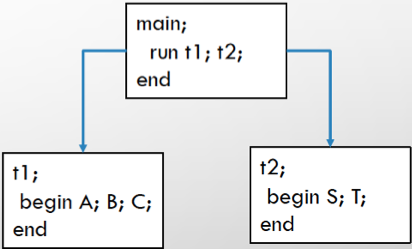
\includegraphics[max size={\textwidth}{\textheight}]{images/chapter-3/concurrent-program-spawing-threads.png}
  \end{minipage}}
  \fbox{\begin{minipage}{\dimexpr \textwidth-2\fboxsep-2\fboxrule}
    \abovecaptionskip=0pt
    \caption{Concurrent program spawning threads $t_{1}$ and $t_{2}$}
  \end{minipage}}
\end{figure}

In this example, the concurrent program spawns the threads $t_{1}$ and $t_{2}$ where:
\begin{longtabu} to \textwidth { X[1.5,l] X[0.2,l] X[3,l]}
	\textbullet $t_{1}$ has three statements & -- &
	A, B and C; and
	\\
	\textbullet $t_{2}$ has two statements & -- &
	S and T.
\end{longtabu}

There are two threads and therefore it is possible to use the adjusted formula to calculate the number of interleavings in this concurrent program:

\begin{equation*}
	\begin{aligned}
		\text{number of interleavings} & = \frac{(n + m)!}{n!m!} \\
		\text{number of interleavings} & = \frac{(3 + 2)!}{3! \times 2!} \\
		\text{number of interleavings} & = \frac{6!}{3! \times 2!} \\
		\text{number of interleavings} & = \frac{6\times5\times4\times3\times2\times1}{(3\times2\times1)\times(2\times1)} \\
		\text{number of interleavings} & = \frac{120}{6\times2} \\
		\text{number of interleavings} & = \frac{120}{12} \\
		\text{number of interleavings} & = 10
	\end{aligned}
\end{equation*}

There are 10 possible interleavings, thus yielding 10 possible different execution sequences.

\begin{figure}[H]
  \lineskip=-\fboxrule
  \fbox{\begin{minipage}{\dimexpr \textwidth-2\fboxsep-2\fboxrule}
    \centering
    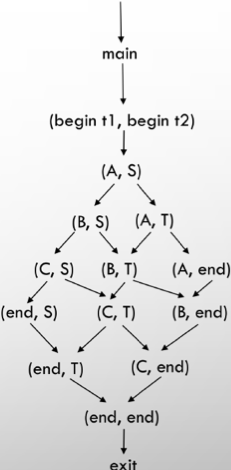
\includegraphics[max size={\textwidth}{\textheight}]{images/chapter-3/possible-execution-sequences.png}
  \end{minipage}}
  \fbox{\begin{minipage}{\dimexpr \textwidth-2\fboxsep-2\fboxrule}
    \abovecaptionskip=0pt
    \caption{Visual representation of the possible execution sequences}
  \end{minipage}}
\end{figure}

A run of the program corresponds to an interleaving sequence. Each interleaving sequence determines a unique sequence of executing the statements. Repeated runs with the same input will likely trace different interleavings.


\subsection*{Growth of interleavings}

The number of interleavings grows extremely quickly given an increase in:
\begin{itemize}
	\item the number of threads in the concurrent program; or
	\item the number of statements/operations in one or more of the concurrent program’s threads.
\end{itemize}

This can be demonstrated by increasing the number of operations in the previous example:
\begin{longtabu} to \textwidth { X[2,l] X[0.2,l] X[3,l]}
	\textbullet $t_{1}$ now has four statements  & -- &
	A, B, C and D; and
	\\
	\textbullet $t_{2}$ now has five statements  & -- &
	S, T, U, V and W.
\end{longtabu}
and therefore:
\begin{equation*}
	\begin{aligned}
		\text{number of interleavings} & = \frac{(n + m)!}{n!m!} \\
		\text{number of interleavings} & = \frac{(4 + 5)!}{4!\times5!} \\
		\text{number of interleavings} & = \frac{9!}{4!\times5!} \\
		\text{number of interleavings} & = \frac{9\times8\times7\times6\times5\times4\times3\times2\times1}{(4\times3\times2\times1)\times(5\times4\times3\times2\times1)} \\
		\text{number of interleavings} & = \frac{362880}{24\times120} \\
		\text{number of interleavings} & = \frac{362880}{2880} \\
		\text{number of interleavings} & = 126
	\end{aligned}
\end{equation*}


\newpage

\section{User and kernel threads}

\section*{User threads}

User threads are created and managed by a user level library, typically without the knowledge of the kernel.

\begin{figure}[H]
  \lineskip=-\fboxrule
  \fbox{\begin{minipage}{\dimexpr \textwidth-2\fboxsep-2\fboxrule}
    \centering
    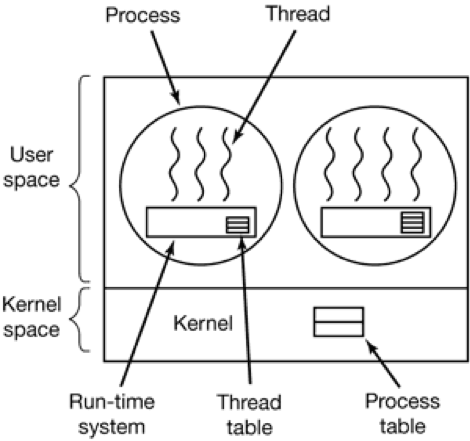
\includegraphics[max size={\textwidth}{\textheight}]{images/chapter-3/user-threads.png}
  \end{minipage}}
  \fbox{\begin{minipage}{\dimexpr \textwidth-2\fboxsep-2\fboxrule}
    \abovecaptionskip=0pt
    \caption{User threads}
  \end{minipage}}
\end{figure}

The diagram shows that:
\begin{itemize}
	\item all of the threads for a given process is present within the user space; and
	\item the thread table is present within the process.
\end{itemize}

User threads are:
\begin{itemize}
	\item fast to create and manage; and
	\item portable to any operating system (OS).
\end{itemize}

If one user thread is blocked, all other threads in the same process are also blocked. For example, in a word processor application, a thread that handles a printing event would block all other threads and therefore prevent the user from interacting with other aspects of the application.

Multi-threaded applications cannot take advantage of parallel execution on computer systems with a multi-core CPU or computer systems with multiple CPUs.


\newpage

\section*{Kernel threads}

Kernel threads are directly managed and supported by the operating system’s (OS’s) kernel.

\begin{figure}[H]
  \lineskip=-\fboxrule
  \fbox{\begin{minipage}{\dimexpr \textwidth-2\fboxsep-2\fboxrule}
    \centering
    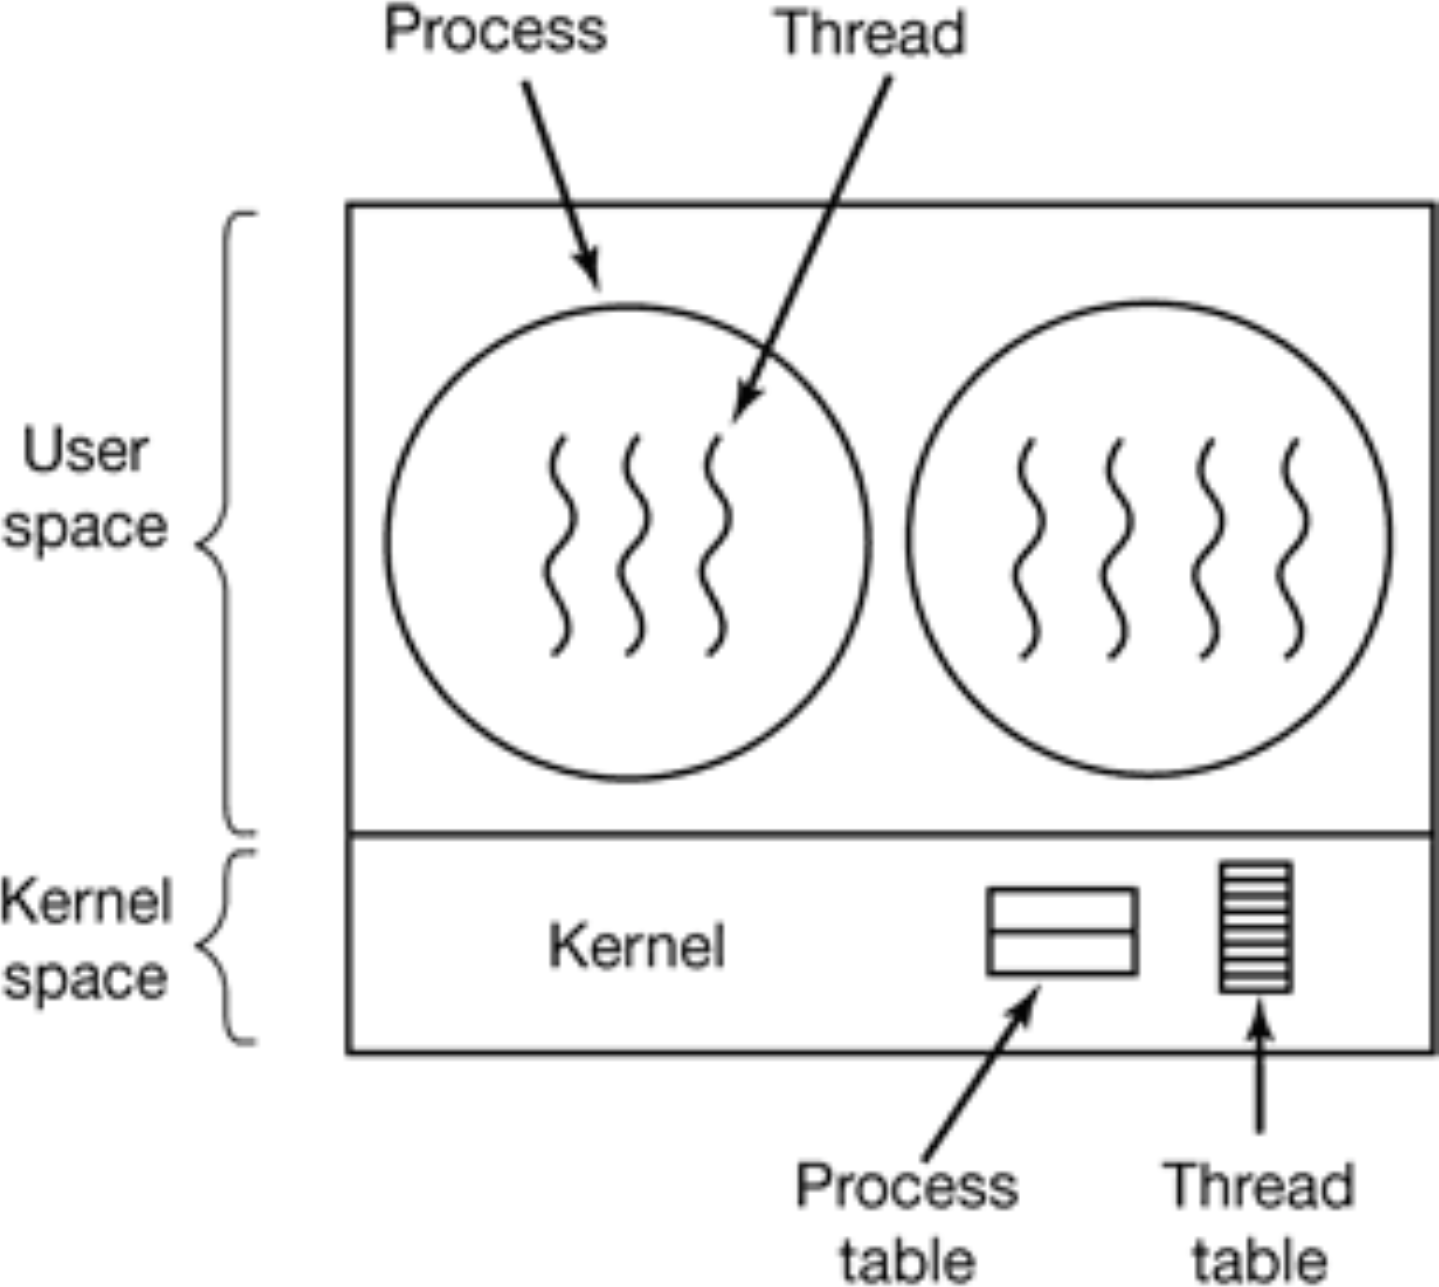
\includegraphics[max size={\textwidth}{\textheight}]{images/chapter-3/kernel-threads.png}
  \end{minipage}}
  \fbox{\begin{minipage}{\dimexpr \textwidth-2\fboxsep-2\fboxrule}
    \abovecaptionskip=0pt
    \caption{Kernel threads}
  \end{minipage}}
\end{figure}

The diagram shows that:
\begin{itemize}
	\item all of the threads for a given process is present within the user space; and
	\item the thread table is present within the kernel space, rather than the process itself or the user space.
\end{itemize}

Kernel threads are:
\begin{itemize}
	\item slower to create and manage than user threads; and
	\item specific to the operating system (OS).
\end{itemize}

If one user thread is blocked, all other threads in the same process are scheduled and not blocked. For example, in a word processor application, a thread that handles a printing event would no longer block all other threads and therefore would allow the user to interacting with other aspects of the application whilst the printing event occurs.

Can take advantage of parallel execution on computer systems with a multi-core CPU or computer systems with multiple CPUs.



\section{Multi-threading models}

\section*{Why is multi-threading mapping required?}

The kernel is generally not aware of the user threads present in a process. Therefore, a thread library must map user threads to kernel threads.


\begin{figure}[H]
  \lineskip=-\fboxrule
  \fbox{\begin{minipage}{\dimexpr \textwidth-2\fboxsep-2\fboxrule}
    \centering
    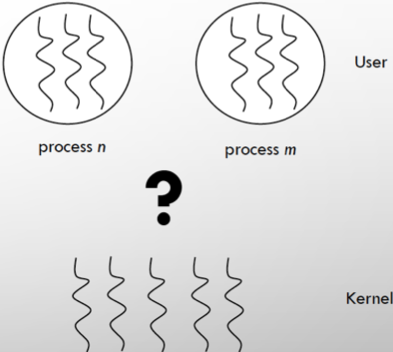
\includegraphics[max size={\textwidth}{\textheight}]{images/chapter-3/multi-threading-mapping.png}
  \end{minipage}}
  \fbox{\begin{minipage}{\dimexpr \textwidth-2\fboxsep-2\fboxrule}
    \abovecaptionskip=0pt
    \caption{Multi-threading mapping}
  \end{minipage}}
\end{figure}

The diagram shows that there must be some relationship between the user threads and the kernel threads. This relationship may defined using different mappings, including:
\begin{itemize}
	\item many-to-one;
	\item one-to-one; and
	\item many-to-many.
\end{itemize}


\section*{Many-to-one mapping}

\subsection*{How it works}

All user threads from each process map to one kernel thread.

\begin{figure}[H]
  \lineskip=-\fboxrule
  \fbox{\begin{minipage}{\dimexpr \textwidth-2\fboxsep-2\fboxrule}
    \centering
    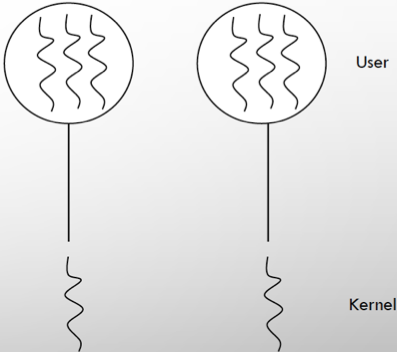
\includegraphics[max size={\textwidth}{\textheight}]{images/chapter-3/many-to-one-mapping.png}
  \end{minipage}}
  \fbox{\begin{minipage}{\dimexpr \textwidth-2\fboxsep-2\fboxrule}
    \abovecaptionskip=0pt
    \caption{Many-to-one mapping}
  \end{minipage}}
\end{figure}


\subsection*{Evalution}

\begin{longtabu} to \textwidth {|X[1,l]|X[1,l]|}
    \hline
    \textbf{Advantages} & \textbf{Disadvantages}
    \\ \hline
    \textbf{Portable} as there are few system dependencies.
    &
    \textbf{No parallel execution of threads}.
    \\ \hline
    &
    \textbf{No concurrency} as all threads in a process are blocked if another thread is blocked, for example if the thread is waiting for an input/output (I/O) interrupt.
	\\ \hline
\end{longtabu}


\section*{One-to-one mapping}

\subsection*{How it works}

Each user thread maps to a single kernel thread.

\begin{figure}[H]
  \lineskip=-\fboxrule
  \fbox{\begin{minipage}{\dimexpr \textwidth-2\fboxsep-2\fboxrule}
    \centering
    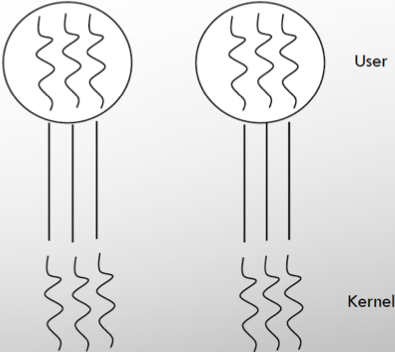
\includegraphics[max size={\textwidth}{\textheight}]{images/chapter-3/one-to-one-mapping.png}
  \end{minipage}}
  \fbox{\begin{minipage}{\dimexpr \textwidth-2\fboxsep-2\fboxrule}
    \abovecaptionskip=0pt
    \caption{One-to-one mapping}
  \end{minipage}}
\end{figure}


\subsection*{Evaluation}

\begin{longtabu} to \textwidth {|X[1,l]|X[1,l]|}
    \hline
    \textbf{Advantages} & \textbf{Disadvantages}
    \\ \hline
    \textbf{Concurrency} as all threads in a process are not blocked if any given thread becomes blocked.
    &
    \textbf{Slow} as there is management overhead because the kernel is involved for every user thread.
    \\ \hline
    \textbf{Performance} as it can take advantage of multiple CPUs.
    &
    \textbf{Restricted} as there is typically a limit on the number of threads.
	\\ \hline
    &
    \textbf{Creating user threads requires the corresponding kernel support}.
	\\ \hline
\end{longtabu}


\section*{Many-to-many mapping}

\subsection*{How it works}

Many user threads multiplex to an equal or smaller number of kernel threads.

\begin{figure}[H]
  \lineskip=-\fboxrule
  \fbox{\begin{minipage}{\dimexpr \textwidth-2\fboxsep-2\fboxrule}
    \centering
    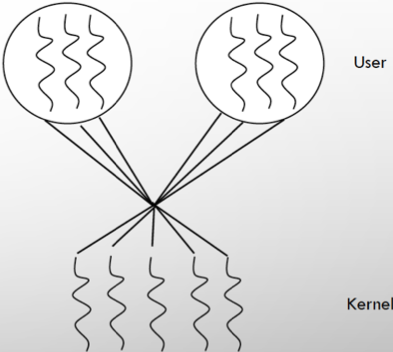
\includegraphics[max size={\textwidth}{\textheight}]{images/chapter-3/many-to-many-mapping.png}
  \end{minipage}}
  \fbox{\begin{minipage}{\dimexpr \textwidth-2\fboxsep-2\fboxrule}
    \abovecaptionskip=0pt
    \caption{Many-to-many mapping}
  \end{minipage}}
\end{figure}

\begin{longtabu} to \textwidth {|X[1,l]|X[1,l]|}
    \hline
    \textbf{Advantages} & \textbf{Disadvantages}
    \\ \hline
    \textbf{Performance} as it can take advantage of multiple CPUs.
    &
    \textbf{Complexity} and therefore implementation difficulties.
    \\ \hline
    \textbf{Flexible} as there is no limit on the number of threads.
    &
	\\ \hline
\end{longtabu}


\newpage

\section{Evaluation of concurrent programming}
\begin{longtabu} to \textwidth {|X[1,l]|X[1,l]|}
    \hline
    \textbf{Advantages} & \textbf{Disadvantages}
    \\ \hline
    \begin{wrapfigure}{l}{4cm}
		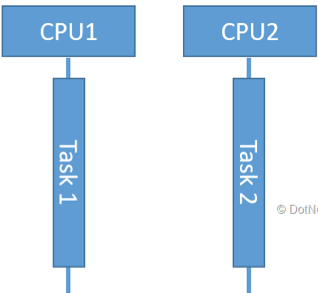
\includegraphics[width=4cm]{images/chapter-3/parallelism.png}
	\end{wrapfigure} 
    \textbf{Parallelism.} It improves the efficiency of program execution in computer systems with multiple CPUs by allows tasks/operations to be split up and executed independently on each CPU.
    &
    \textbf{Debugging complexity} as concurrent programs are non-deterministic and therefore it can be difficult to trace a problem/bug in the code as the same input will generally not result in the same output.  
    \\ \hline
    \begin{wrapfigure}{l}{0.8cm}
		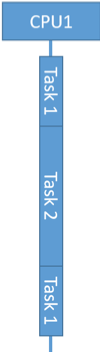
\includegraphics[width=0.8cm]{images/chapter-3/multi-tasking.png}
	\end{wrapfigure}
    \textbf{Multi-tasking.} It improves the utilisation of the CPU in a computer system that only has a single CPU. This allows multiple tasks/operations to run alongside each other and appear to be processed simultaneously.
    &
    \textbf{No protection between threads}.
    \\ \hline
    \textbf{Increases application responsiveness}, for example, in a word processor application one thread could be responsible for responding to user input/output (I/O) while other threads perform tasks in the background.
    &
    \textbf{Concurrent processes must interact with each other} in order to share resources or exchange data.
    \\ \hline
    \textbf{Suited to some applications} as there are some practical applications that are non-deterministic and concurrent as the order of program operations is determined by other external events. This is useful for applications that need to handle multiple events.
    &
    \textbf{Synchronisation must be promoted} in order to determine when, how and with what language abstractions computation events can be synchronised in order to eliminate unacceptable outputs.
    \\ \hline
    &
    \textbf{Distribution must be taken care of} in order to consider how threads can be distributed among a number of CPUs and how one thread is able to interact with another thread on a different CPU.
    \\ \hline
    &
    \textbf{Error-prone}.
	Examples of major concurrent programming errors include:
	\begin{itemize}
		\item Therac-25	- A computerised radiation therapy machine whose errors contributed to accidents causing deaths and serious injuries.
		\item Mars Rover Pathfinder	– Problems with interaction between concurrent tasks caused periodic software resets, thus reducing availability for exploration.
	\end{itemize}
	\\ \hline
\end{longtabu}


\chapter{Memory Management}

\section{Race condition}

\section*{Definition}

A \textbf{race condition} describes the competition for resources in a critical section caused by interleaving/thread interference.


\section*{Why do race conditions happen?}

Race conditions occur due to interleaving/thread interference.

\textbf{Interleaving/thread interference} describes an undesired outcome resulting from non-deterministic, concurrent usage of shared resources.

This happens because, in general, concurrent execution is non-deterministic, and therefore the same input generally means different output due to ordering. This is because there are many cases where the order of operation does matter.


\section*{Examples}

\subsection*{Racing for memory access}

A race condition may occur when two threads attempt to access the same location memory, such as registers or RAM, at the same time.

\begin{figure}[H]
  \lineskip=-\fboxrule
  \fbox{\begin{minipage}{\dimexpr \textwidth-2\fboxsep-2\fboxrule}
    \centering
    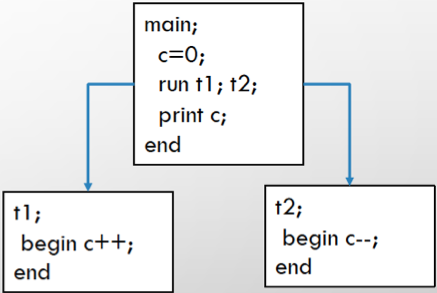
\includegraphics[max size={\textwidth}{\textheight}]{images/chapter-4/concurrent-program-spawning-threads.png}
  \end{minipage}}
  \fbox{\begin{minipage}{\dimexpr \textwidth-2\fboxsep-2\fboxrule}
    \abovecaptionskip=0pt
    \caption{Concurrent program spawning threads $t_{1}$ and $t_{2}$}
  \end{minipage}}
\end{figure}

In this example, the two threads $t_{1}$ and $t_{2}$ manipulate the same variable where:
\begin{itemize}
	\item $t_{1}$ increments the variable $c$; and
	\item $t_{2}$ decrements the variable $c$.
\end{itemize}

As seen before (page 40), each statement may be compiled in to several machine instructions.

The increment ($c++$) instruction is broken in to three machine instructions:
\begin{itemize}
	\item retrieve $c$;
	\item increment retrieved value; and
	\item store result in $c$.
\end{itemize}

The decrement ($c--$) instruction is also broken in to three machine instructions:
\begin{itemize}
	\item retrieve $c$;
	\item decrement retrieved value; and
	\item store result in $c$.
\end{itemize}

As a result, one interleaving possibility is as follows:
\begin{itemize}
	\item $t_{1}$: retrieve $c$;
	\item $t_{2}$: retrieve $c$;
	\item $t_{1}$: increment retrieved value; (result is $1$)
	\item $t_{2}$: decrement retrieved value; (result is $-1$)
	\item $t_{1}$: store result in $c$; ($c$ is now 1)
	\item $t_{2}$: store result in $c$; ($c$ is now -1)
\end{itemize}

This example shows that the race condition has caused the result from thread $t_{1}$ to be lost as it has been overwritten by the result from thread $t_{2}$.


\subsection*{Racing for peripheral access}

A race condition may also occur when two threads attempt to access the same peripheral, such as a printer spooler directory, at the same time.

\begin{figure}[H]
  \lineskip=-\fboxrule
  \fbox{\begin{minipage}{\dimexpr \textwidth-2\fboxsep-2\fboxrule}
    \centering
    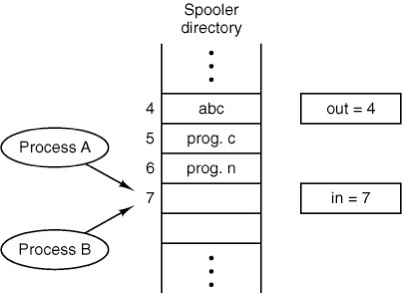
\includegraphics[max size={\textwidth}{\textheight}]{images/chapter-4/printer-spooler-directory.png}
  \end{minipage}}
  \fbox{\begin{minipage}{\dimexpr \textwidth-2\fboxsep-2\fboxrule}
    \abovecaptionskip=0pt
    \caption{Printer spooler directory}
  \end{minipage}}
\end{figure}

In this example, the two processes $A$ and $B$ attempt to access the printer spooler directory at the same time:
\begin{itemize}
	\item the next available printer job slot is $7$;
	\item process $A$ and $B$ access printer job slot $7$ simultaneously;
	\item process $A$ reads printer job slot $7$ and a timer interrupt occurs that causes a context switch to process $B$ before process $A$ has opportunity to store any data;
	\item process $B$ reads printer job slot $7$ and stores its job data and increments the values; and
	\item another timer interrupt occurs that causes a context switch to process $A$ that then stores its job at printer job slot $7$.
\end{itemize}

This example shows that the race condition has caused the job data stored in the printer spooler directory by process $B$ to be lost as it has been overwritten by the job data from process $A$.


\section{Inter-process synchronisation}

\section*{Definition}

\textbf{Inter-process synchronisation} involves techniques that are designed to prevent race conditions and allows threads/processes to share resources.


\section*{Behaviour of threads}

Threads in a computer system may behave in two possible ways:
\begin{itemize}
	\item competing -- two or more processes compete for the same computing resource, for example access to a particular memory cell; or
	\item cooperating -- two or more processes may need to communicate with one another, thus causing information to be passed from one to the other.
\end{itemize}

Inter-process synchronisation is required to manage both threads that are competing and threads that are cooperating.

An operating system (OS) itself contains both threads that are competing and threads that are cooperating.


\section*{How mutual exclusion works}

The solution to preventing race conditions is by implementing mutual exclusion on any given critical section/region.

The \textbf{critical section/region} is code in a process that involves sensitive operations on a shared resource.

\textbf{Mutual exclusion} is the requirement that one thread of execution never enters its critical section/region at the same time that another concurrent thread of execution enters its own critical section/region.

\begin{figure}[H]
  \lineskip=-\fboxrule
  \fbox{\begin{minipage}{\dimexpr \textwidth-2\fboxsep-2\fboxrule}
    \centering
    \includegraphics[max size={\textwidth}{\textheight}]{images/chapter-4/mutual-exclusion.png}
  \end{minipage}}
  \fbox{\begin{minipage}{\dimexpr \textwidth-2\fboxsep-2\fboxrule}
    \abovecaptionskip=0pt
    \caption{Mutual exclusion on critical section/region}
  \end{minipage}}
\end{figure}

When a thread/process enters its critical section/region, no other thread/process may also enter its critical section/region. 

This is demonstrated in the diagram above:
\begin{itemize}
	\item at time interval $T_{1}$, process $A$ enters its critical section/region;
	\item at time interval $T_{2}$, process $B$ attempts to enter its critical section/region;
	\item process $B$ is blocked from entering its critical section/region until process $A$ leaves its critical section/region;
	\item at time interval $T_{3}$, process $A$ leaves its critical section/region and therefore process $B$ is allowed to enter its critical section/region; and
	\item at time interval $T_{4}$, process $B$ leaves its critical section/region.
\end{itemize}

This shown that mutual exclusion is enforced as no two threads/processes are simultaneously inside their critical sections/regions.

For mutual exclusion to be effective:
\begin{itemize}
	\item no assumptions may be made about the speeds or the number of threads/processes;
	\item no threads/processes running outside its critical section/region may block other threads/processes, such that a thread/process that is not in its critical section/region cannot prevent other threads from entering their critical section/region; and
	\item no thread/process should have to wait forever to enter its critical section/region.
\end{itemize}

Mutual exclusion is a major design issue in operating systems (OSs) as consideration must be taken in order to prevent race conditions while maintaining parallelism and efficiency.


\section*{How mutual exclusion is implemented}

Mutual exclusion is implemented using semaphores.

A \textbf{semaphore} is a system tool used for the design of correct synchronisation protocols. This was introduced by Edsger Dijkstra in the 1962/1963. Semaphores are implemented using a variable or abstract data type and are used to control thread/process access to a resource. They are typically integer values that accept only non-negative values.

\begin{figure}[H]
  \lineskip=-\fboxrule
  \fbox{\begin{minipage}{\dimexpr \textwidth-2\fboxsep-2\fboxrule}
    \centering
    \includegraphics[max size={\textwidth}{\textheight}]{images/chapter-4/semaphore-interaction.png}
  \end{minipage}}
  \fbox{\begin{minipage}{\dimexpr \textwidth-2\fboxsep-2\fboxrule}
    \abovecaptionskip=0pt
    \caption{Semaphore interaction on critical section/region}
  \end{minipage}}
\end{figure}

The diagram shows that semaphores allow the CPU to context switch between threads/processes when one becomes blocked.

It is convenient to write entry and exit protocols using a single atomic statement. This statement is atomic and therefore is indivisible, meaning that the statement cannot be interrupted.

As mentioned before, a semaphore, denoted by $S$, is an integer that takes only non-negative values. Only two atomic (indivisible) statements are permitted, as shown below.

\begin{longtabu*} to \textwidth {|X[0.5,l]|X[1,l]|X[1,l]|}
    \hline
	\textbf{Statement} & \textbf{Statement Implementation}
	& \textbf{Usage}
	\\ \hline
	$wait(s)$
	&
	\begin{verbatim}
	wait(s)
	{
	    if ( S > 0 )
	    {
	        S--;
	    }
	}
	\end{verbatim}
	&
	If a thread/process is in its non-critical section/region and wishes to enter its critical section/region, this statement will be performed.

	This means that the thread/process will be blocked until $S = 0$
	evaluates to $True$.
	\\ \hline
	$signal(s)$
	&
	\begin{verbatim}
	signal(s)
	{
	    S++;
	}
	\end{verbatim}
	&
	If a thread/process is in its critical section/region, this statement will be performed.

	This helps to achieve mutual exclusion as it prevents $S = 0$ from evaluating to $True$ until the thread/process has left its critical section/region.
	\\ \hline
\end{longtabu*}

This is a good solution as there is no possibility for a race condition as these statements will always be enforced due to the face that they are atomic (indivisible) statements and cannot be interrupted.


\section{The producer-consumer problem}

\section*{Problem description}

The producer-consumer problem is a classical inter-process communication problem in which:
\begin{itemize}
	\item a producer repeatedly produces items and places them in to a buffer; and
	\item a consumer consumes the items one-by-one by taking them from the buffer.
\end{itemize}

This problem has the following requirements:
\begin{itemize}
	\item the buffer must be assumed to be first in, first out (FIFO);
	\item the producer may produce a new item only at a time when the buffer is not full;
	\item the consumer may consume an item only at a time when the buffer is not empty; and
	\item the process terminates when all items produced are eventually consumed.
\end{itemize}

\begin{figure}[H]
  \lineskip=-\fboxrule
  \fbox{\begin{minipage}{\dimexpr \textwidth-2\fboxsep-2\fboxrule}
    \centering
    \includegraphics[max size={\textwidth}{\textheight}]{images/chapter-4/producer-consumer-problem.png}
  \end{minipage}}
  \fbox{\begin{minipage}{\dimexpr \textwidth-2\fboxsep-2\fboxrule}
    \abovecaptionskip=0pt
    \caption{The producer-consumer problem}
  \end{minipage}}
\end{figure}

The problem arises when attempting to devise a method that is able to:
\begin{itemize}
	\item put the producer to “sleep” when the buffer is full to prevent further items being produced when there is no space in the buffer; and
	\item “wake” the consumer when the buffer is not empty as there is possibility to consumer when the buffer is not empty.
\end{itemize}


\section*{Possible solution}

This problem could be solved by keeping track of the number of items in the buffer.

This could be achieved by implementing loops in the producer class and consumer class.

\newpage

\begin{lstlisting}[title={Producer class}]
LOOP
{
	Produce item i         //produce item
	if ( itemCount == N )  //end of buffer
	{
		sleep(producer);
	}

	Put item i;            // place item in to buffer
	itemCount++;           // increment buffer count
	if ( itemCount == 1)   // buffer nearly empty
	{
		wakeup(consumer);
	}
}
\end{lstlisting}

\begin{lstlisting}[title={Consumer class}]
LOOP
{
	if ( itemCount == 0 )    // buffer empty
	{
		sleep(consumer);
	}

	Remove item j;           // remove item from buffer
	itemCount--;             // decrement buffer count
	if ( itemCount == N-1 )  // buffer has space
	{
		wakeup(producer);
	}
	Consume item j;          // consume item
}
\end{lstlisting}

The loop in the producer class would be running as one thread and the loop in the consumer thread would be running as another thread. These two threads would be running in parallel. As a result, if the threads in the solution are interleaved, a race condition may occur, which in turn, may cause a deadlock.


\subsection*{Deadlocks}

A \textbf{deadlock} occurs when two or more threads wait for each other to finish.

Four conditions must be hold simultaneously in order for a deadlock to occur:
\begin{itemize}
	\item mutual exclusion -- a resource can be assigned to, at most, one process at a time;
	\item hold and wait -- processes holding resources are permitted to request and wait for additional resources;
	\item no pre-emption	 -- resources previously locked cannot be forcefully unlocked by another process, instead they must be released by the holding process; and
	\item circular wait -- there must be a chain of processes, such that each member of the chain is waiting for a resource held by the next member of the chain, as shown in the diagram below.
\end{itemize}

\begin{figure}[H]
  \lineskip=-\fboxrule
  \fbox{\begin{minipage}{\dimexpr \textwidth-2\fboxsep-2\fboxrule}
    \centering
    \includegraphics[max size={\textwidth}{\textheight}]{images/chapter-4/circular-wait.png}
  \end{minipage}}
  \fbox{\begin{minipage}{\dimexpr \textwidth-2\fboxsep-2\fboxrule}
    \abovecaptionskip=0pt
    \caption{Circular wait}
  \end{minipage}}
\end{figure}

A deadlock may occur in the possible solution described previously.

\begin{figure}[H]
  \lineskip=-\fboxrule
  \fbox{\begin{minipage}{\dimexpr \textwidth-2\fboxsep-2\fboxrule}
    \centering
    Consumer reads $itemCount = 0$ and it evaluates to $True$, and therefore $sleep(consumer)$ needs to be called.
    
	$\downarrow$
	
	Just before $sleep(consumer)$ is called, the consumer is interrupted by a timer interrupt and the producer is resumed.
	
	$\downarrow$
	
	The producer places an item in to the buffer, such that $itemCount = 1$.
	
	$\downarrow$
	
	The producer tries to perform $wakeup(consumer)$ however, the consumer is already in “wakeup” mode. As a result, the call to $wakeup(consumer)$ is missed.
	
	$\downarrow$
	
	When the consumer resumes, it will call $sleep(consumer)$ and get trapped in “sleep” mode.
	
	$\downarrow$
	
	The producer will continue placing items in the buffer and call $sleep(producer)$ when the buffer is full.
	
	$\downarrow$
	
	There is now a deadlock as both threads are waiting for a $wakeup$ call from each other.
  \end{minipage}}
  \fbox{\begin{minipage}{\dimexpr \textwidth-2\fboxsep-2\fboxrule}
    \abovecaptionskip=0pt
    \caption{Possible deadlock}
  \end{minipage}}
\end{figure}

This possible deadlock shows that another solution is required to effectively solve the producer-consumer problem.


\section*{Solving the problem using semaphores}

It is assumed that
\begin{lstlisting}
ItemsReady = 0
SpacesLeft = N  //size of buffer
\end{lstlisting}

\begin{lstlisting}[title={Producer class}]
LOOP
{
	Produce item i      // produce item
	Wait(SpacesLeft)    // decrement semaphore

	Put item i;         // place item in to buffer
	Signal(ItemsReady)  // increment
}
\end{lstlisting}

\begin{lstlisting}[title={Consumer class}]
LOOP
{
	Wait(ItemsReady)    // decrement semaphore

	Get item j;         // remove item from buffer
	Signal(SpacesLeft)  // increment semaphore
	Consume item i;     // consume item
}
\end{lstlisting}

If this solution uses semaphores correctly, then
\begin{equation*}
	\begin{aligned}
		\text{N = SpacesLeft + ItemsReady}
	\end{aligned}
\end{equation*}

as the producer will always be placing items in to the buffer when there are spaces available in the buffer.

However, this solution does not consider situations in which there are multiple producers and/or multiple consumers.


\newpage

\section*{The multiple producer-consumer problem}

\subsection*{Problem description}

The multiple producer-consumer problem is a classical inter-process communication problem in which:
\begin{itemize}
	\item multiple producer repeatedly produces items and places them in to a buffer; and
	\item multiple consumer consumes the items one-by-one by taking them from the buffer.
\end{itemize}

As with the previous producer-consumer problem, this problem has the following requirements:
\begin{itemize}
	\item the buffer must be assumed to be first in, first out (FIFO);
	\item the producers may produce a new item only at a time when the buffer is not full;
	\item the consumers may consume an item only at a time when the buffer is not empty; and
	\item the process terminates when all items produced are eventually consumed.
\end{itemize}

\begin{figure}[H]
  \lineskip=-\fboxrule
  \fbox{\begin{minipage}{\dimexpr \textwidth-2\fboxsep-2\fboxrule}
    \centering
    \includegraphics[max size={\textwidth}{\textheight}]{images/chapter-4/multiple-producer-consumer-problem.png}
  \end{minipage}}
  \fbox{\begin{minipage}{\dimexpr \textwidth-2\fboxsep-2\fboxrule}
    \abovecaptionskip=0pt
    \caption{The multiple producer-consumer problem}
  \end{minipage}}
\end{figure}

The problem arises when attempting to devise a method that is able to manage:
\begin{itemize}
	\item two producers placing items in to the same slot in the buffer; and
	\item two consumers removing items from the same slot in the buffer.
\end{itemize}
This is similar to the problem discussed in the printer spooler example (page n).

A race condition may also occur when producers attempt to access a variable at the same time.

To demonstrate the race condition, it is necessary to consider the following possible interleaving of the threads/processes:
\begin{itemize}
	\item two producers access the $SpacesLeft$ variable at the same time, which corresponds to decrementing the semaphore;
	\item both producers get the same next empty slot in the buffer at the same time; and
	\item both producers write in to the same slot.
\end{itemize}

This example shows that the race condition has caused the data stored in the buffer slot by the first producer to be lost as it has been overwritten by the data stored in the buffer slot by the second producer.

In order to ensure mutual exclusion when multiple users are involved, an additional semaphore must be introduced.


\subsection*{Mutex}

A \textbf{mutex} (or \textbf{binary semaphore}) is a semaphore with ownership that can only be released by its owner and is initially set to $1$.


\subsection*{Problem solution}

It is now possible to construct a solution, using a mutex (or binary semaphore), that will ensure mutual exclusion even when there are multiple producers and/or multiple consumers.

It is assumed that
\begin{lstlisting}
ItemsReady = 0
SpacesLeft = N  //size of buffer
\end{lstlisting}

\begin{lstlisting}[title={Producer class}]
LOOP
{
	Produce item i      // produce item
	Wait(SpacesLeft)    // decrement semaphore
	Wait(BusyBuffer)    // mutex

	Put item i;         // place item in to buffer
	Signal(BusyBuffer)  // release mutex
	Signal(ItemsReady)  // increment
}
\end{lstlisting}

\begin{lstlisting}[title={Consumer class}]
LOOP
{
	Wait(ItemsReady)    // decrement semaphore
    Wait(BusyBuffer)    // mutex

    Get item j;         // remove item from buffer
    Signal(SpacesLeft)  // increment semaphore
    Signal(BusyBuffer)  // release mutex
    Consume item i;     // consume item
}
\end{lstlisting}

The mutex $BusyBuffer$ has ownership and therefore can only be incremented/decremented by the same thread/process.

The order in which semaphores are incremented and decremented is essential. This can be demonstrated by inspecting the effect of switching around two statements in the Consumer class:
\begin{lstlisting}
Wait(ItemsReady)  //decrement semaphore
Wait(BusyBuffer)  //mutex
...
Wait(BusyBuffer)  //mutex
Wait(ItemsReady)  //decrement semaphore
\end{lstlisting}

This switching would cause …

\end{document}
